\documentclass{beamer}
%% \documentclass[draft]{beamer} %% draft version

%% restrict generation of slides
%% \includeonlyframes{oligoarray,probesyn}

\mode<presentation>
{
  \usetheme{Bielefeld}
  \setbeamercovered{transparent}
}

\usepackage[english]{babel}
\usepackage[latin1]{inputenc}
\usepackage{graphicx}

\usepackage{lmodern}
\usepackage[T1]{fontenc}

\newcommand{\ignore}[1]{}

\title[GCB 2006 - Microarray Layout and the Quadratic Assignment Problem] % (optional, use only with long paper titles)
{Microarray Layout and\\the Quadratic Assignment Problem}

%% \subtitle
%% {Include Only If Paper Has a Subtitle}

\author[S.~A.~de~Carvalho~Jr. (Universit\"at Bielefeld)] % (optional, use only with lots of authors)
{S\'ergio A. de Carvalho Jr.\inst{1,}\inst{2}\inst{,3} \and Sven Rahmann\inst{1,}\inst{2}}
% - Give the names in the same order as the appear in the paper.
% - Use the \inst{?} command only if the authors have different
%   affiliation.

\institute[Universit\"{a}t Bielefeld] % (optional, but mostly needed)
{
\inst{1}%
Algorithms and Statistics for Systems Biology, Genome Informatics,\\
Technische Fakult\"at, Universit\"at Bielefeld, Germany
\and
\inst{2}%
International NRW Graduate School in Bioinformatics and Genome Research
\and
\inst{3}%
Graduiertenkolleg Bioinformatik
}
% - Use the \inst command only if there are several affiliations.
% - Keep it simple, no one is interested in your street address.

\date[GCB 2006] % (optional, should be abbreviation of conference name)
{German Conference on Bioinformatics, 2006}
% - Either use conference name or its abbreviation.
% - Not really informative to the audience, more for people (including
%   yourself) who are reading the slides online

% \subject{Theoretical Computer Science}
% This is only inserted into the PDF information catalog. Can be left
% out. 

% If you have a file called "university-logo-filename.xxx", where xxx
% is a graphic format that can be processed by latex or pdflatex,
% resp., then you can add a logo as follows:

% \pgfdeclareimage[height=0.5cm]{university-logo}{university-logo-filename}
% \logo{\pgfuseimage{university-logo}}

% Delete this, if you do not want the table of contents to pop up at
% the beginning of each subsection:
\AtBeginSubsection[]
{
  \begin{frame}<beamer>
    \frametitle{Outline}
    \tableofcontents[currentsection,hideallsubsections]
  \end{frame}
}

% If you wish to uncover everything in a step-wise fashion, uncomment
% the following command: 
%\beamerdefaultoverlayspecification{<+->}


\begin{document}

%%%%%%%%%%%%%%%%%%%%%%%%%%%%%%%%%%%%%%%%%%%%%%%%%%%%%%%%%%%%%%%%%%%%%%%%%%%%%%%%
\frame[plain]{

  \vspace*{0.4cm}
  \centerline{
    
\includegraphics[height=1.3cm]{pics/aggi_logo.jpg}
    \hspace*{0.6cm}
    
\includegraphics[height=1.3cm]{pics/gsbg_logo.jpg}
  }
  
  \titlepage
}

%%%%%%%%%%%%%%%%%%%%%%%%%%%%%%%%%%%%%%%%%%%%%%%%%%%%%%%%%%%%%%%%%%%%%%%%%%%%%%%%
\frame{\frametitle{Outline}

  \tableofcontents[hideallsubsections]

}

%% *****************************************************************************
\section[Introduction]{Introduction to Microarray Layout}
\subsection{Dummy}
%% *****************************************************************************

%%%%%%%%%%%%%%%%%%%%%%%%%%%%%%%%%%%%%%%%%%%%%%%%%%%%%%%%%%%%%%%%%%%%%%%%%%%%%%%%
\frame[label=oligoarray]{\frametitle{High-Density Oligonucleotide Microarrays}

  \centerline{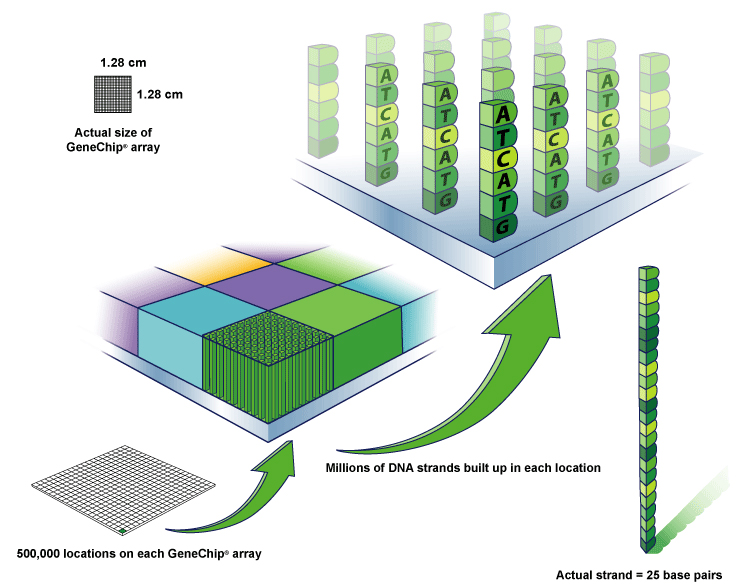
\includegraphics[height=0.9\textheight]{pics/oligoarray.jpg}}
  \vspace*{-0.5cm}
  \centerline{\tiny{Source: Affymetrix, Inc.}}

}

%%%%%%%%%%%%%%%%%%%%%%%%%%%%%%%%%%%%%%%%%%%%%%%%%%%%%%%%%%%%%%%%%%%%%%%%%%%%%%%%
\frame[label=probesyn]{\frametitle{Probe Synthesis with Photolitographic Masks}

  \vspace*{-0.5cm}
  \flushright{\tiny{Source: Affymetrix, Inc.}}
  \centerline{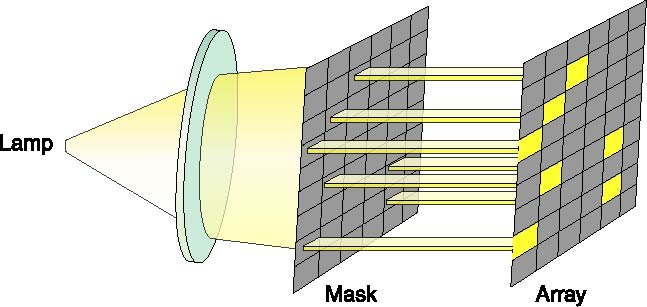
\includegraphics[height=0.5\textheight]{pics/photolithography.jpg}}  

  \begin{itemize}
    \item Probes are synthesized on the chip in a \alert{series of steps}
    \item Each step \alert{appends a particular nucleotide} to selected regions
    \item Selection occurs by exposure to light directed by a \alert{mask}
  \end{itemize}
}

%%%%%%%%%%%%%%%%%%%%%%%%%%%%%%%%%%%%%%%%%%%%%%%%%%%%%%%%%%%%%%%%%%%%%%%%%%%%%%%%
\frame[label=embed]{\frametitle{Deposition Sequence and Probe Embeddings}

  \begin{overprint}
  \onslide<+>
    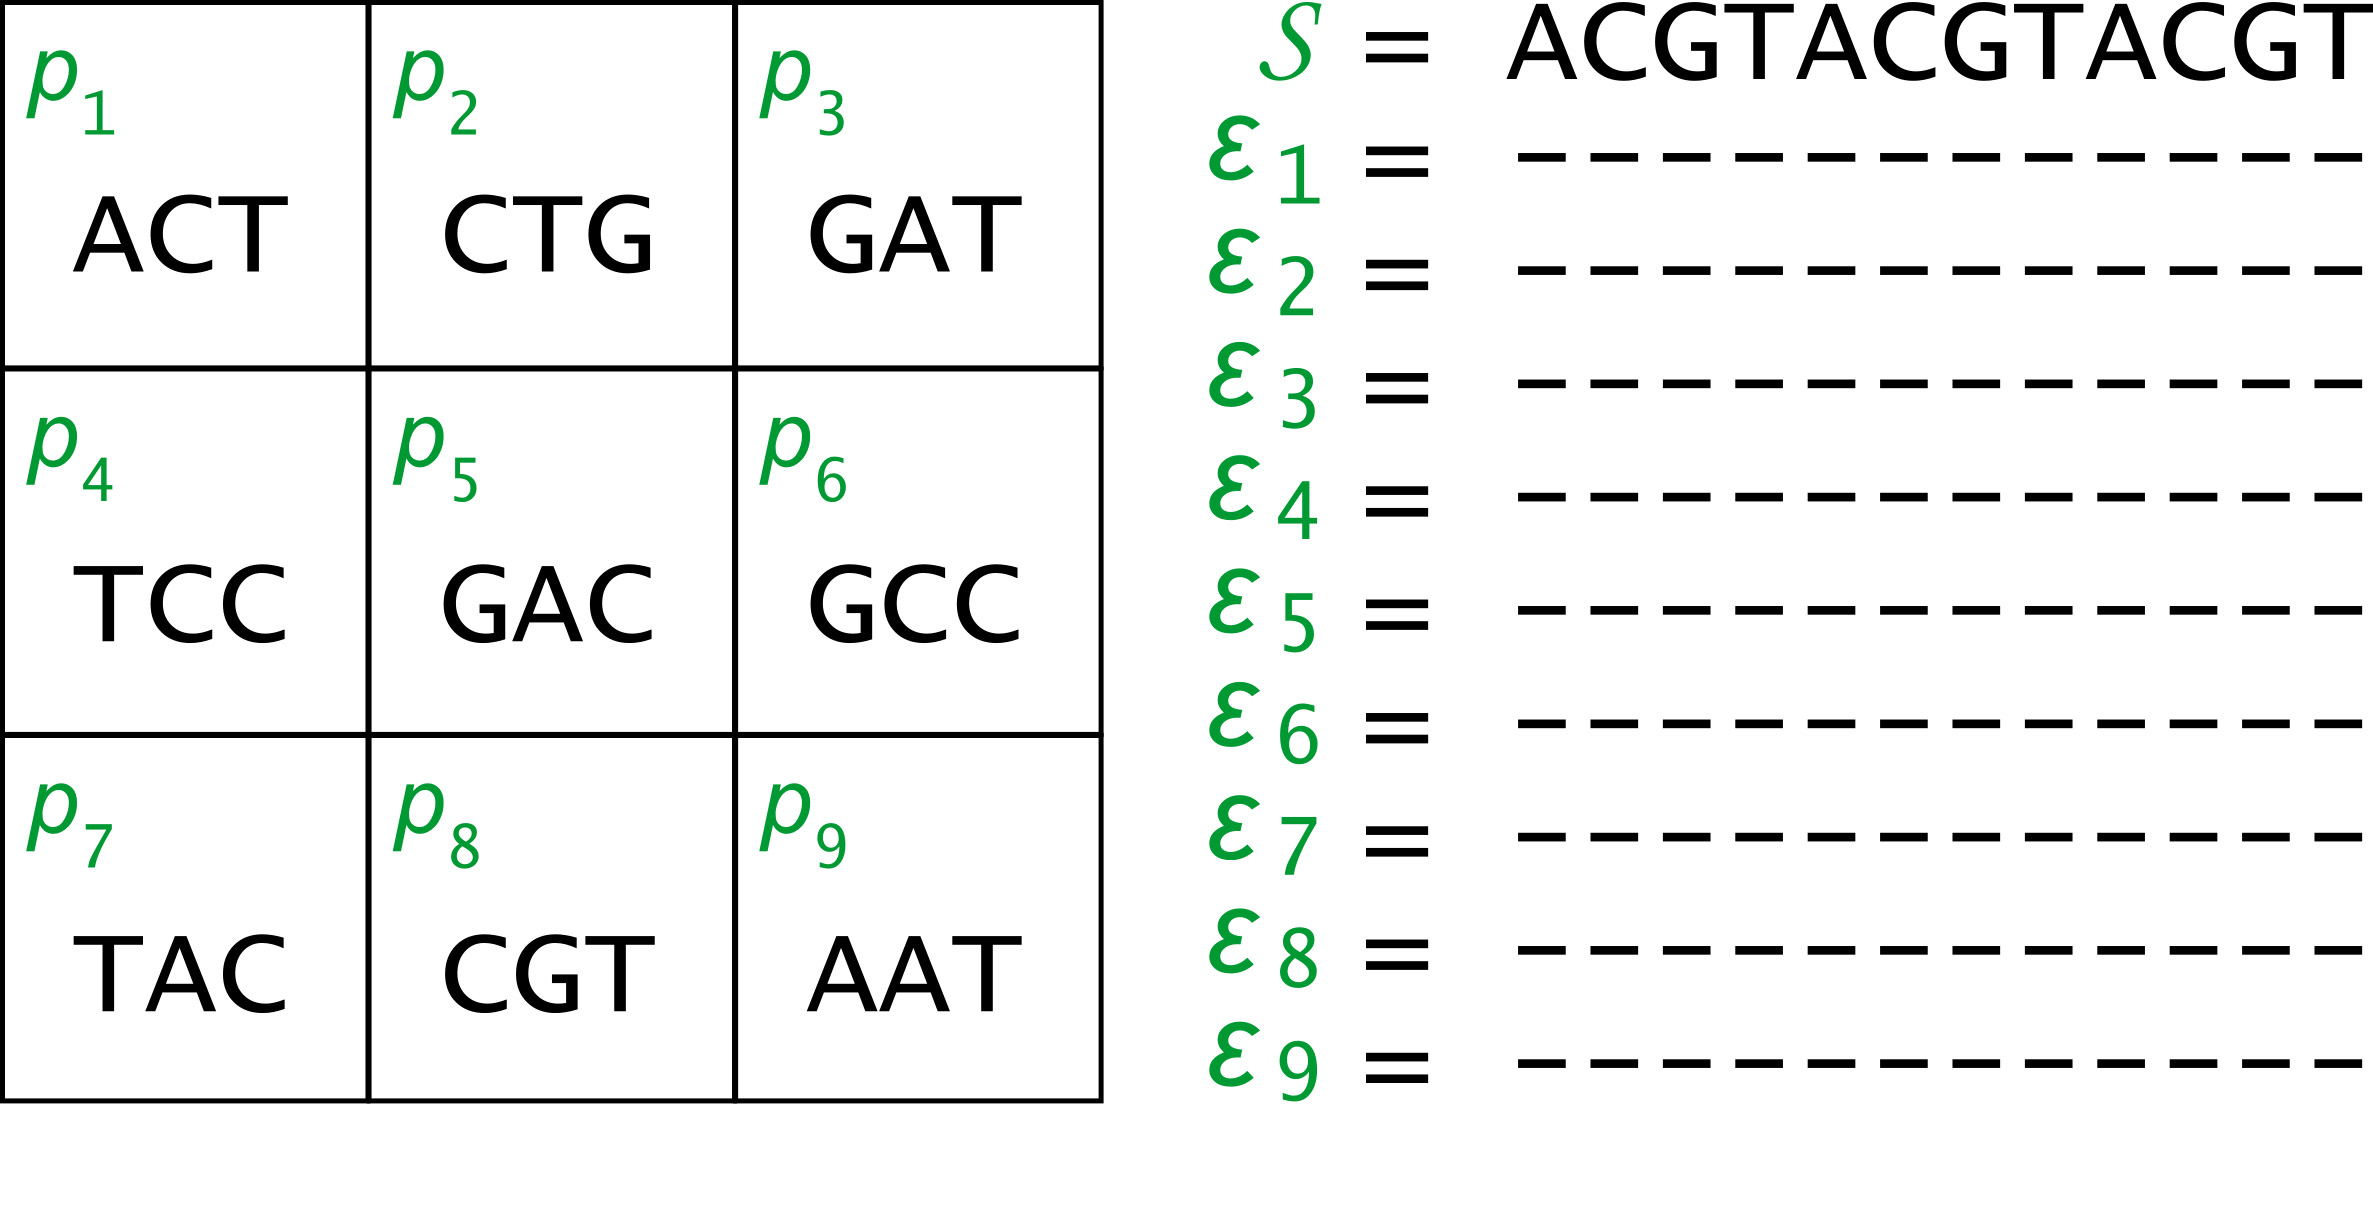
\includegraphics[width=\textwidth]{masks/chip.jpg}
  \onslide<+>
    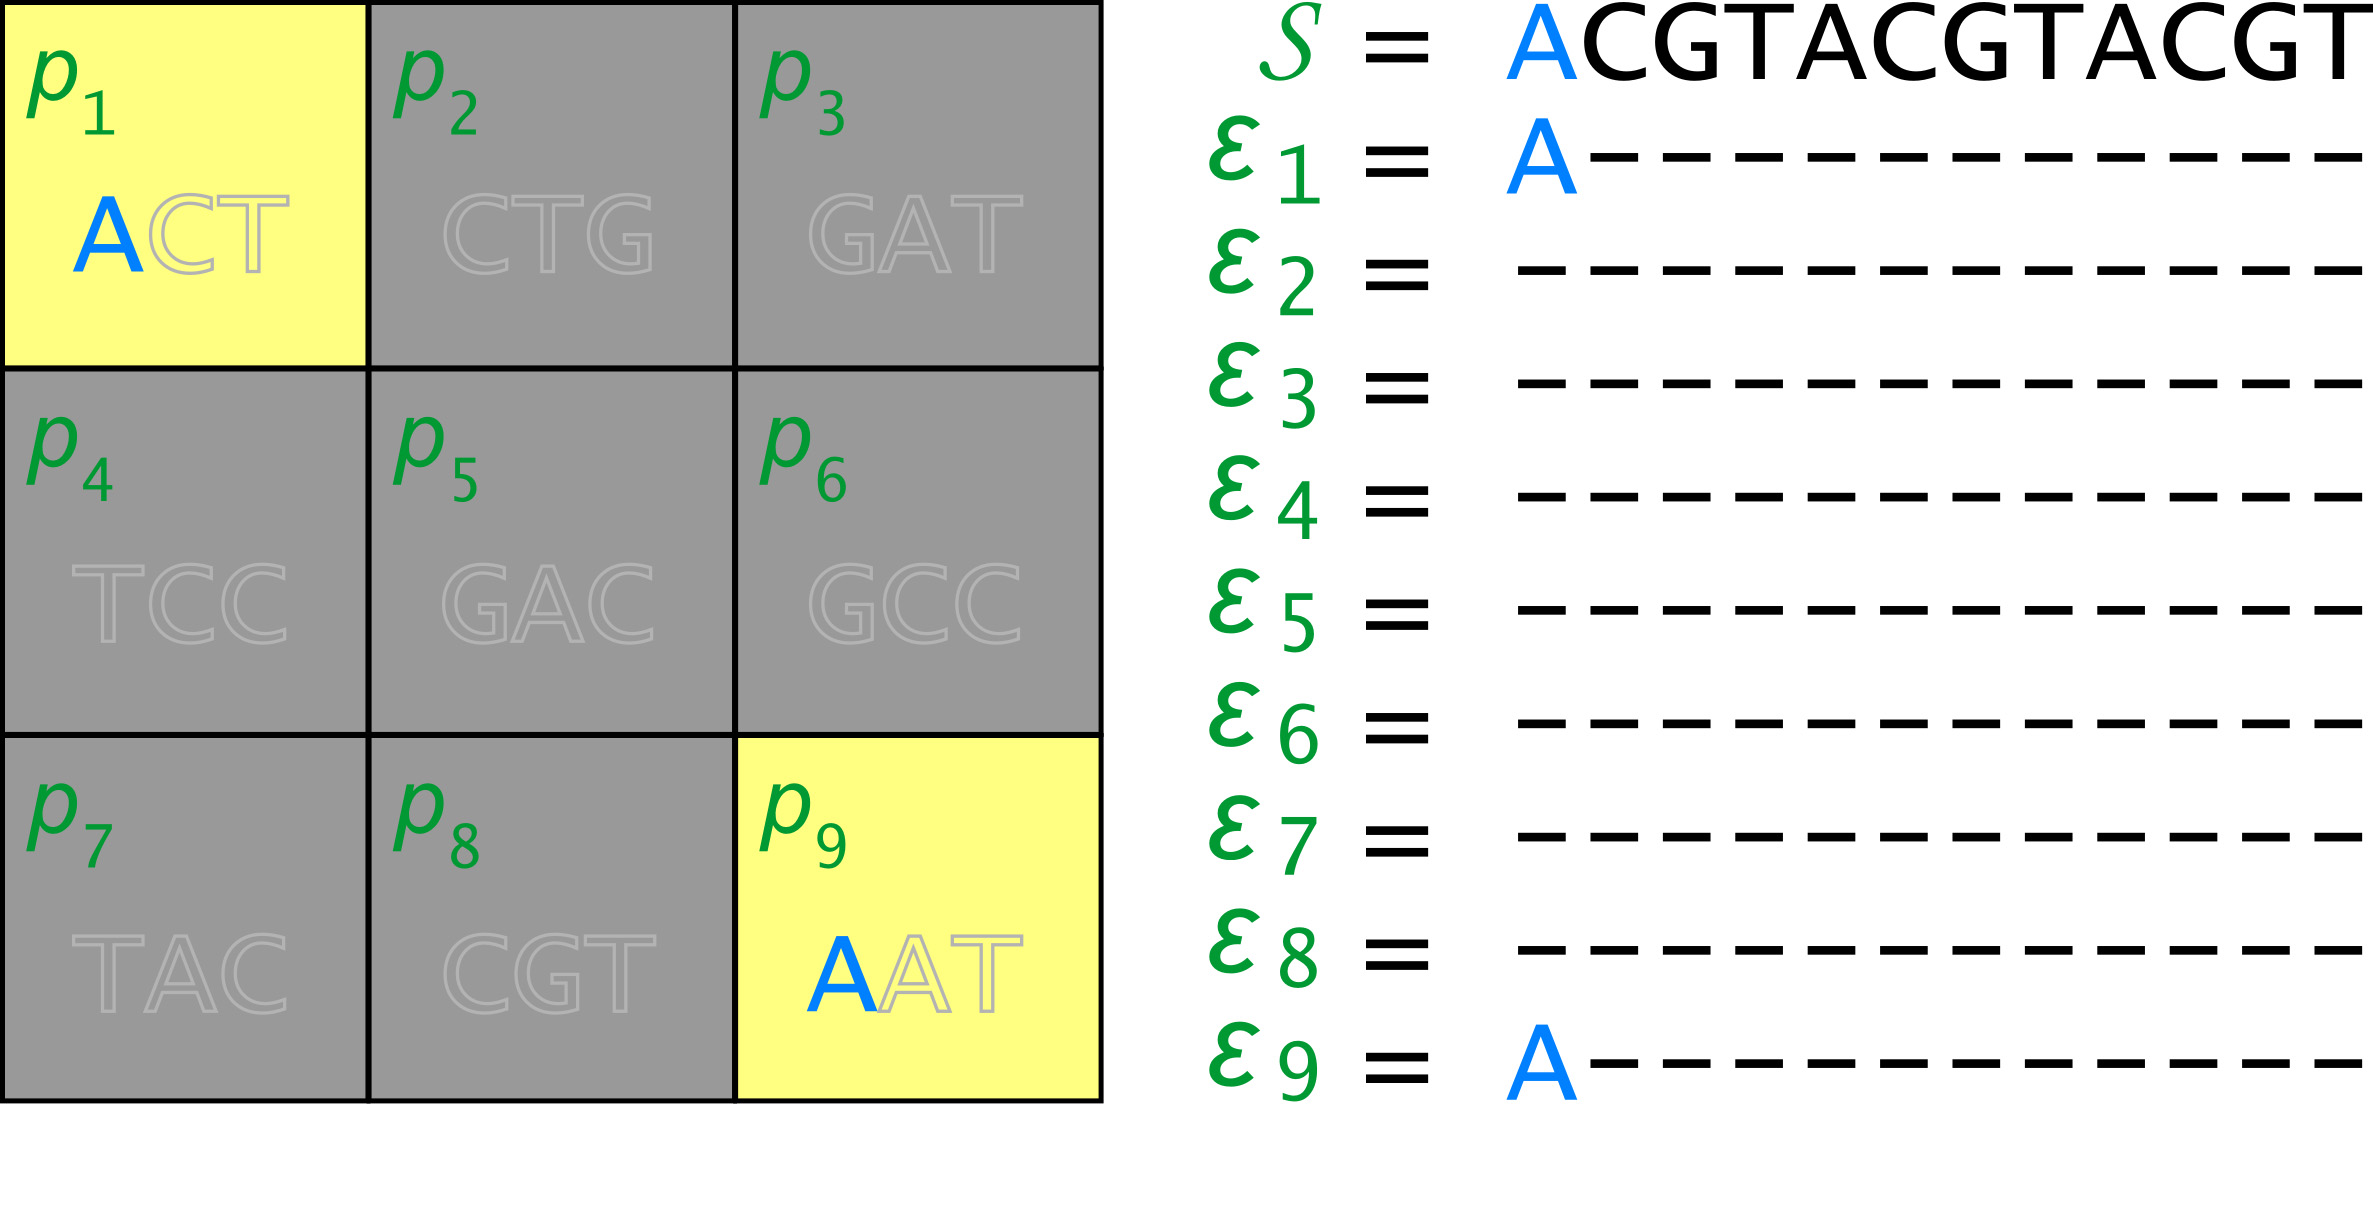
\includegraphics[width=\textwidth]{masks/mask1.jpg}
  \onslide<+>
    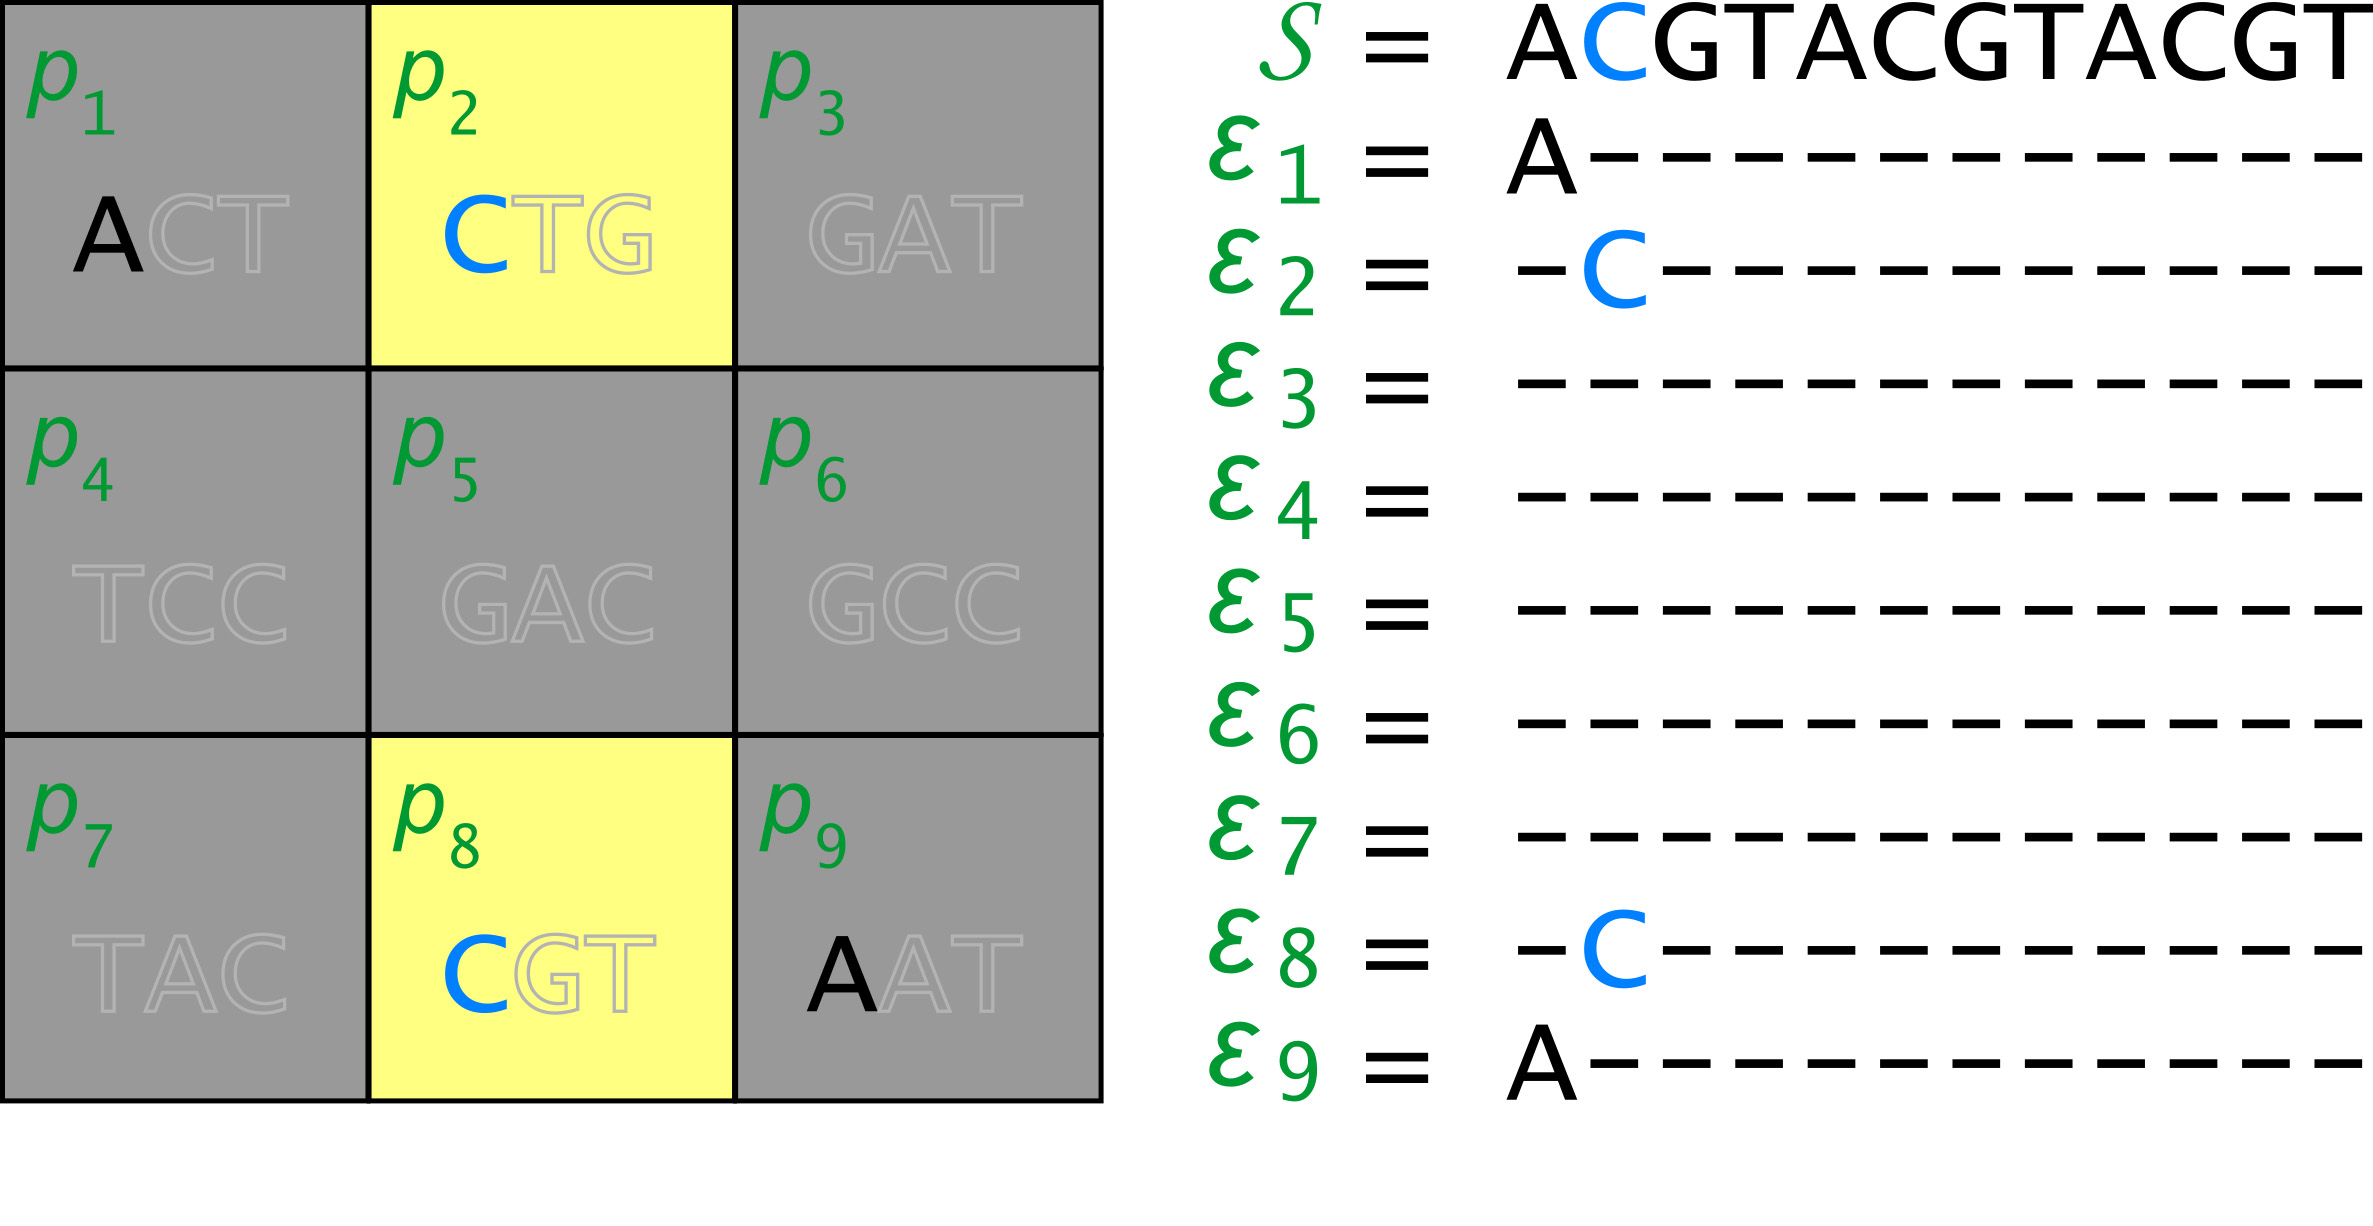
\includegraphics[width=\textwidth]{masks/mask2.jpg}
  \onslide<+>
    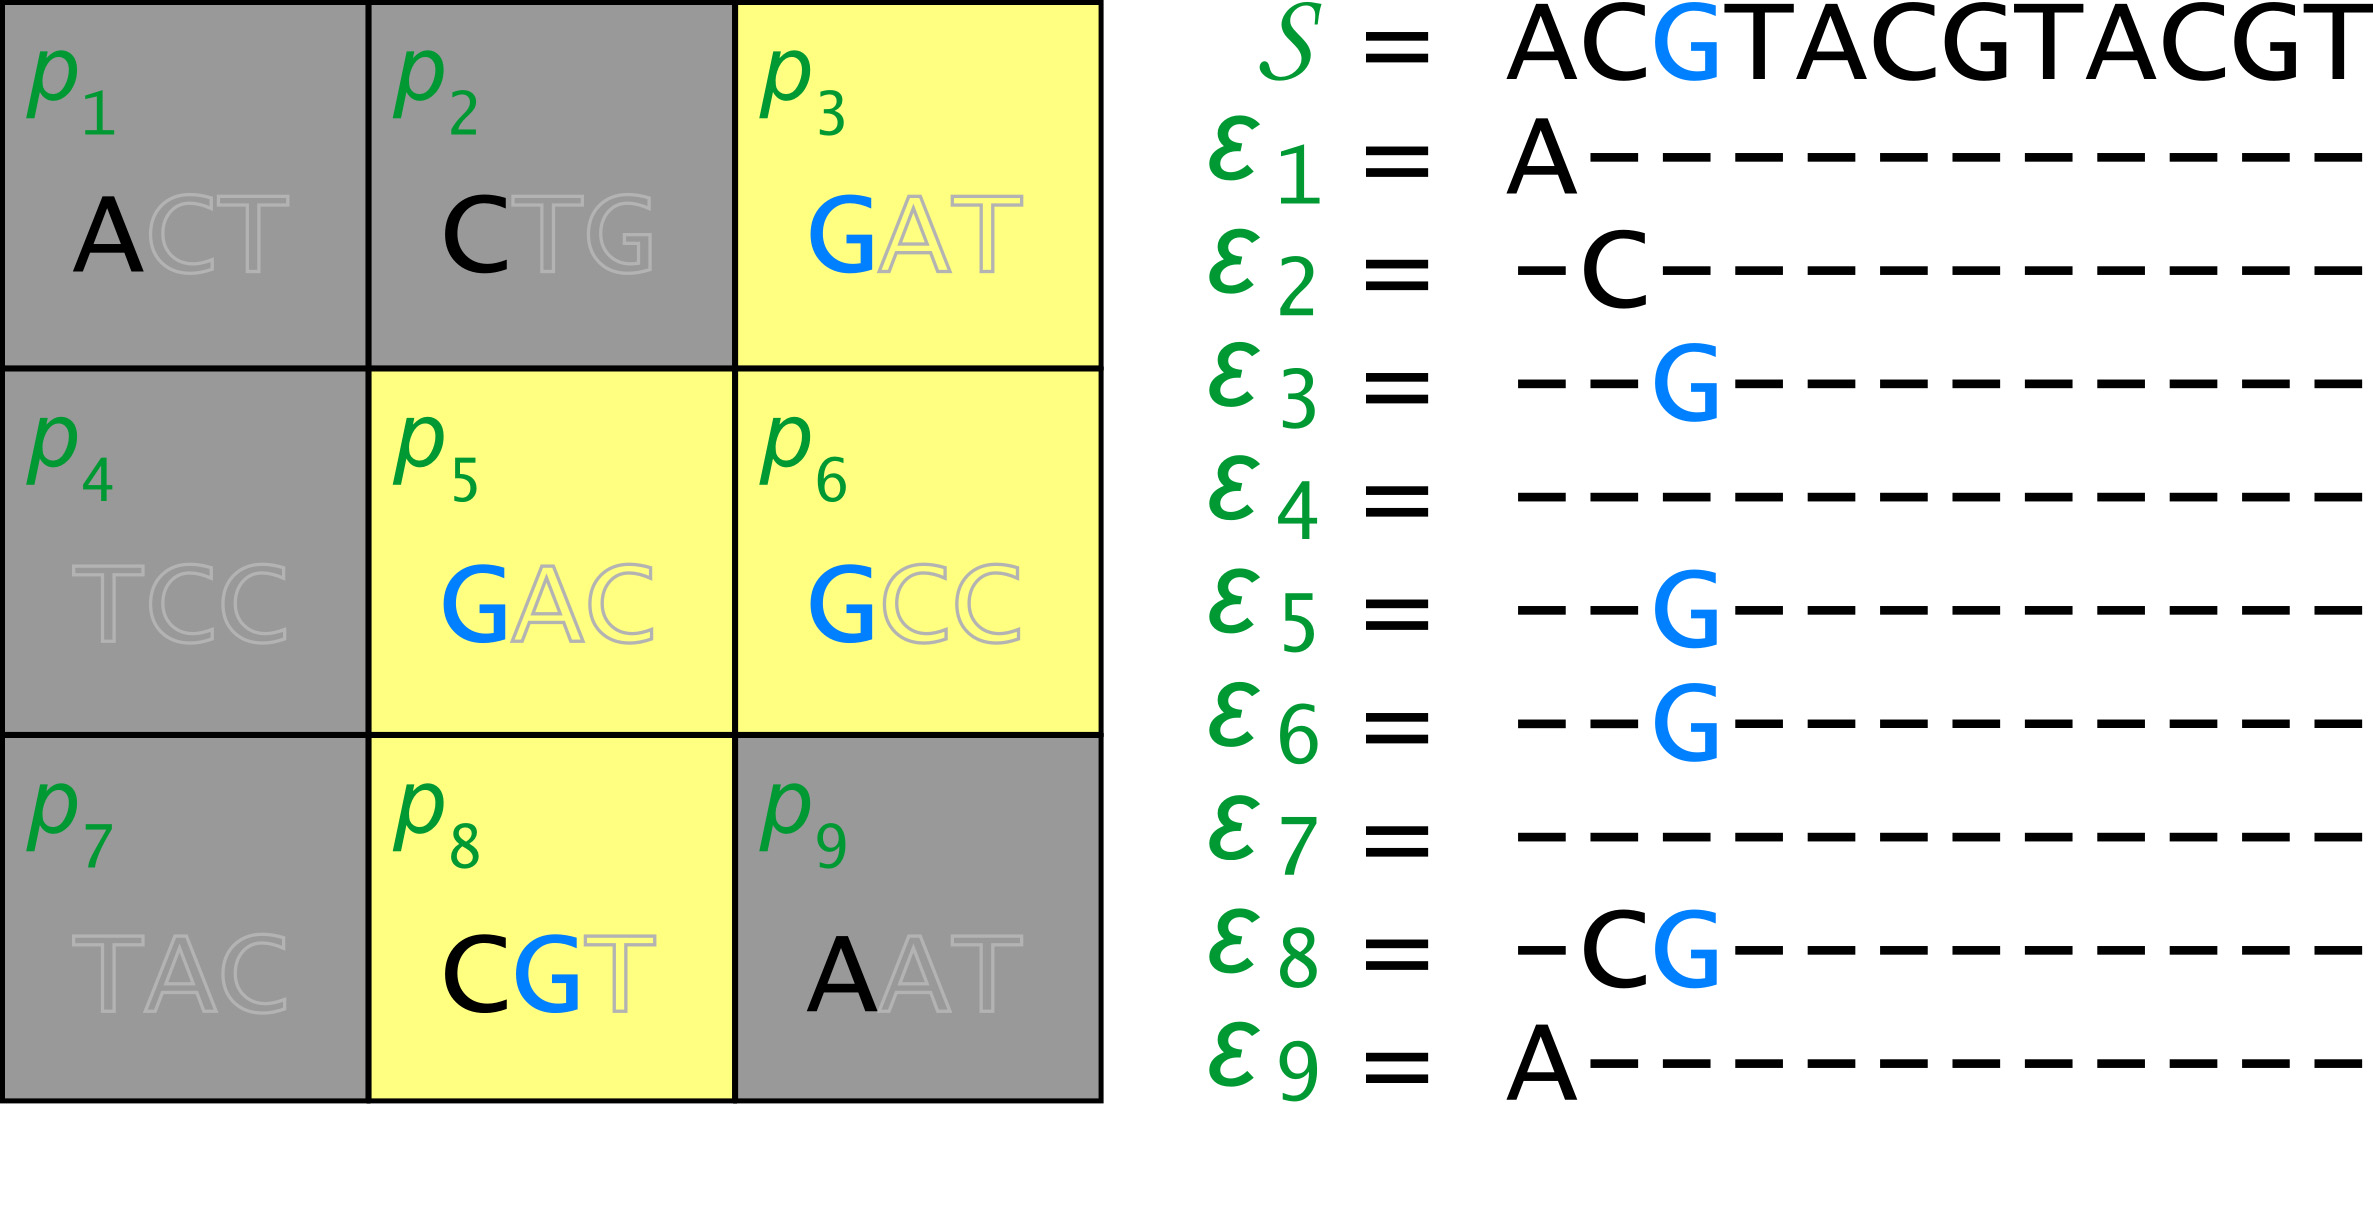
\includegraphics[width=\textwidth]{masks/mask3.jpg}
  \onslide<+>
    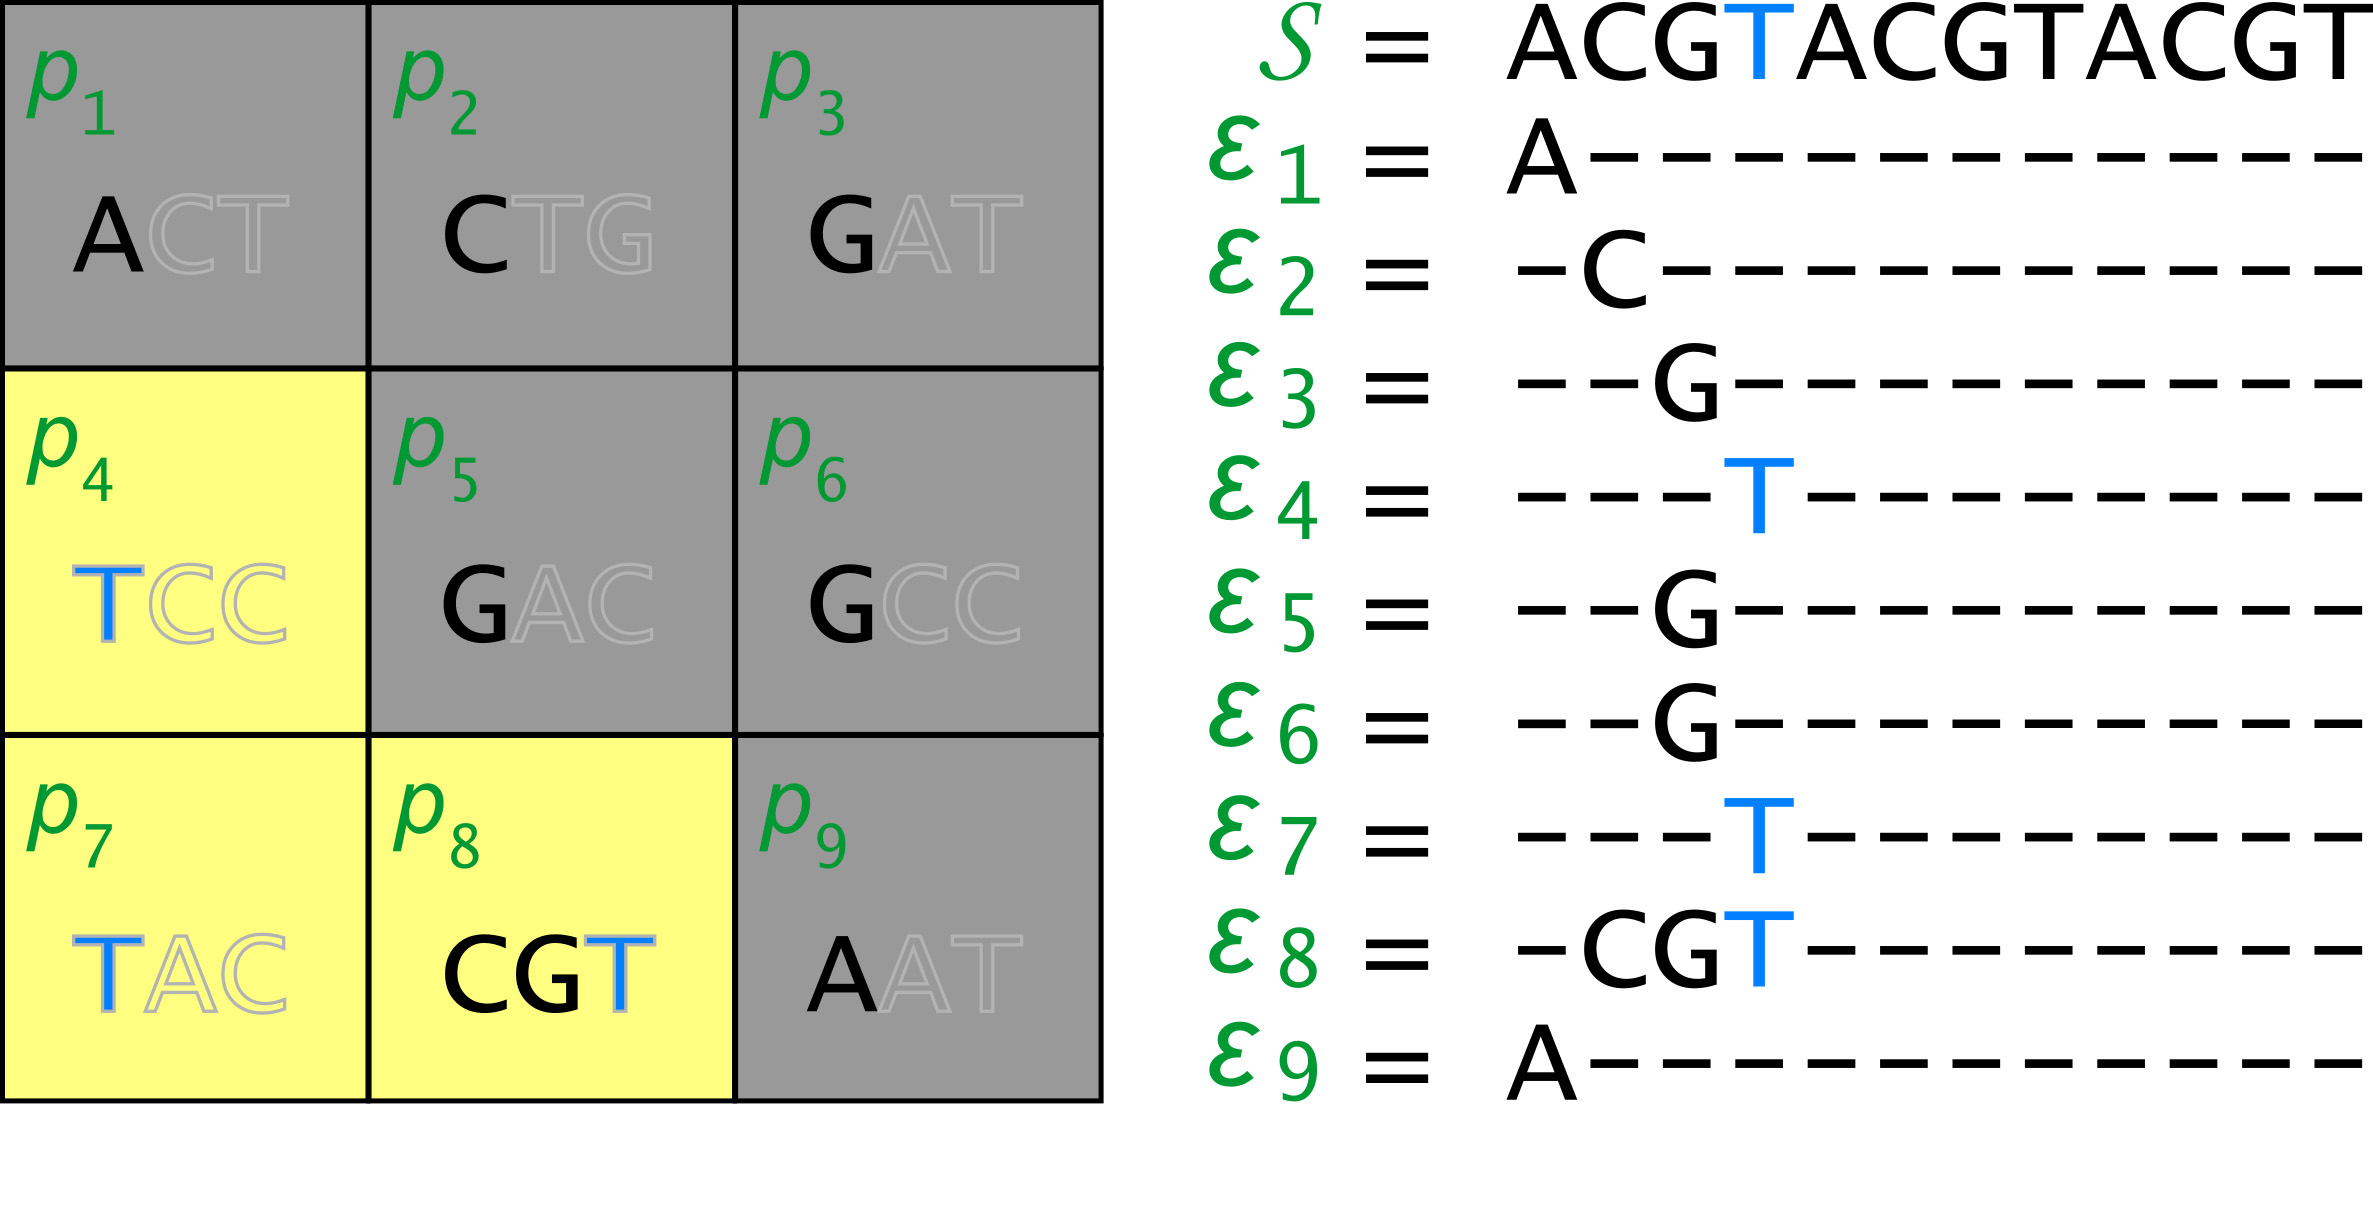
\includegraphics[width=\textwidth]{masks/mask4.jpg}
  \onslide<+>
    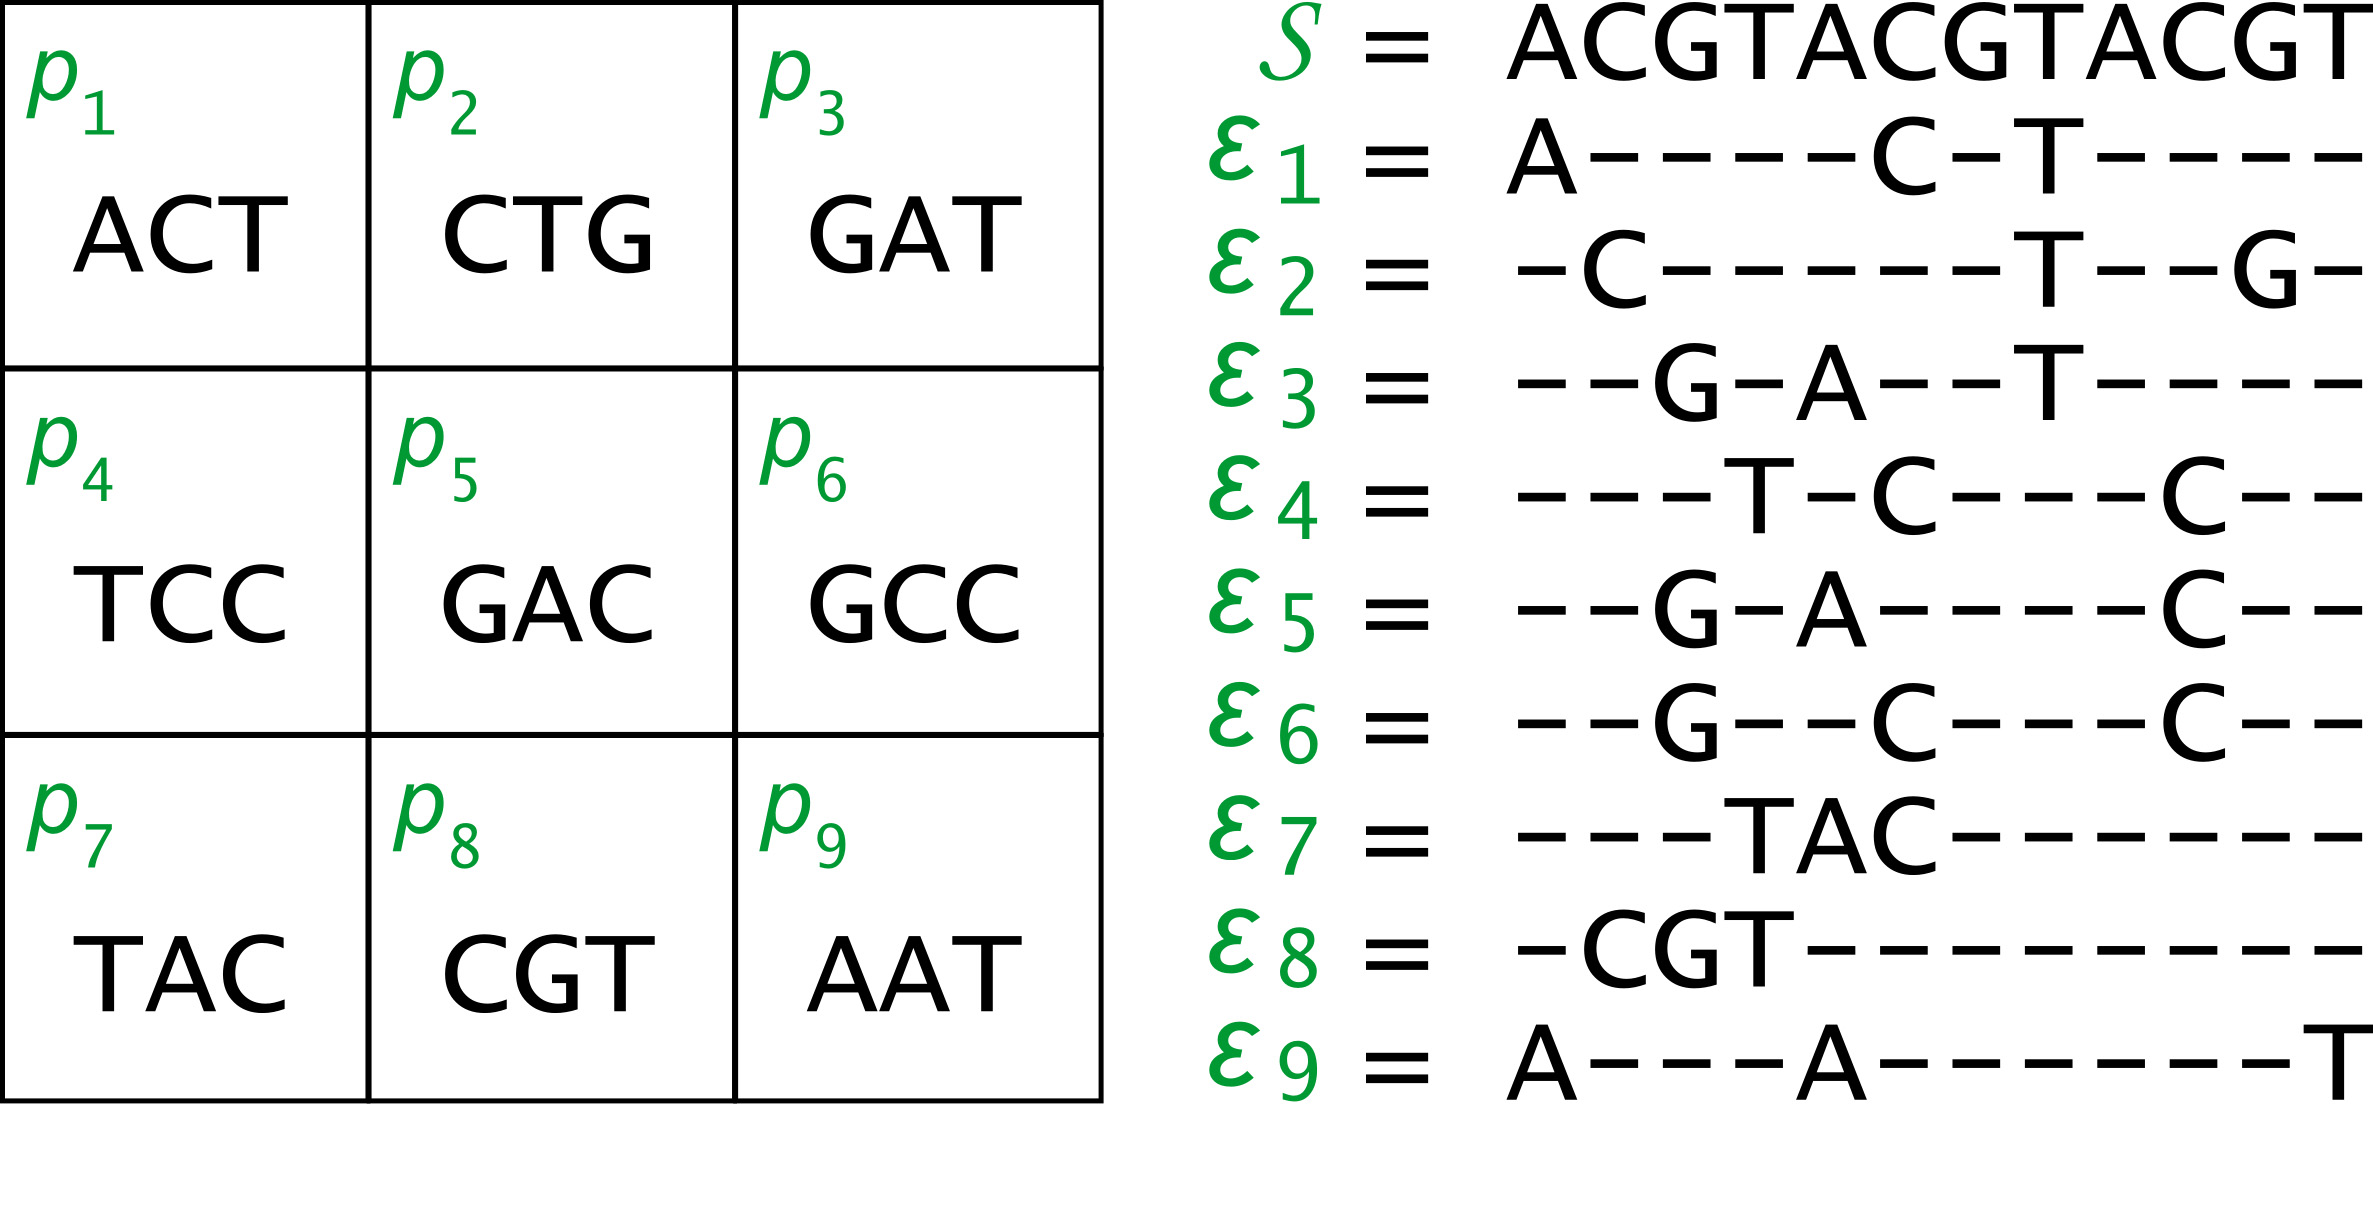
\includegraphics[width=\textwidth]{masks/embed.jpg}
  \onslide<+>
    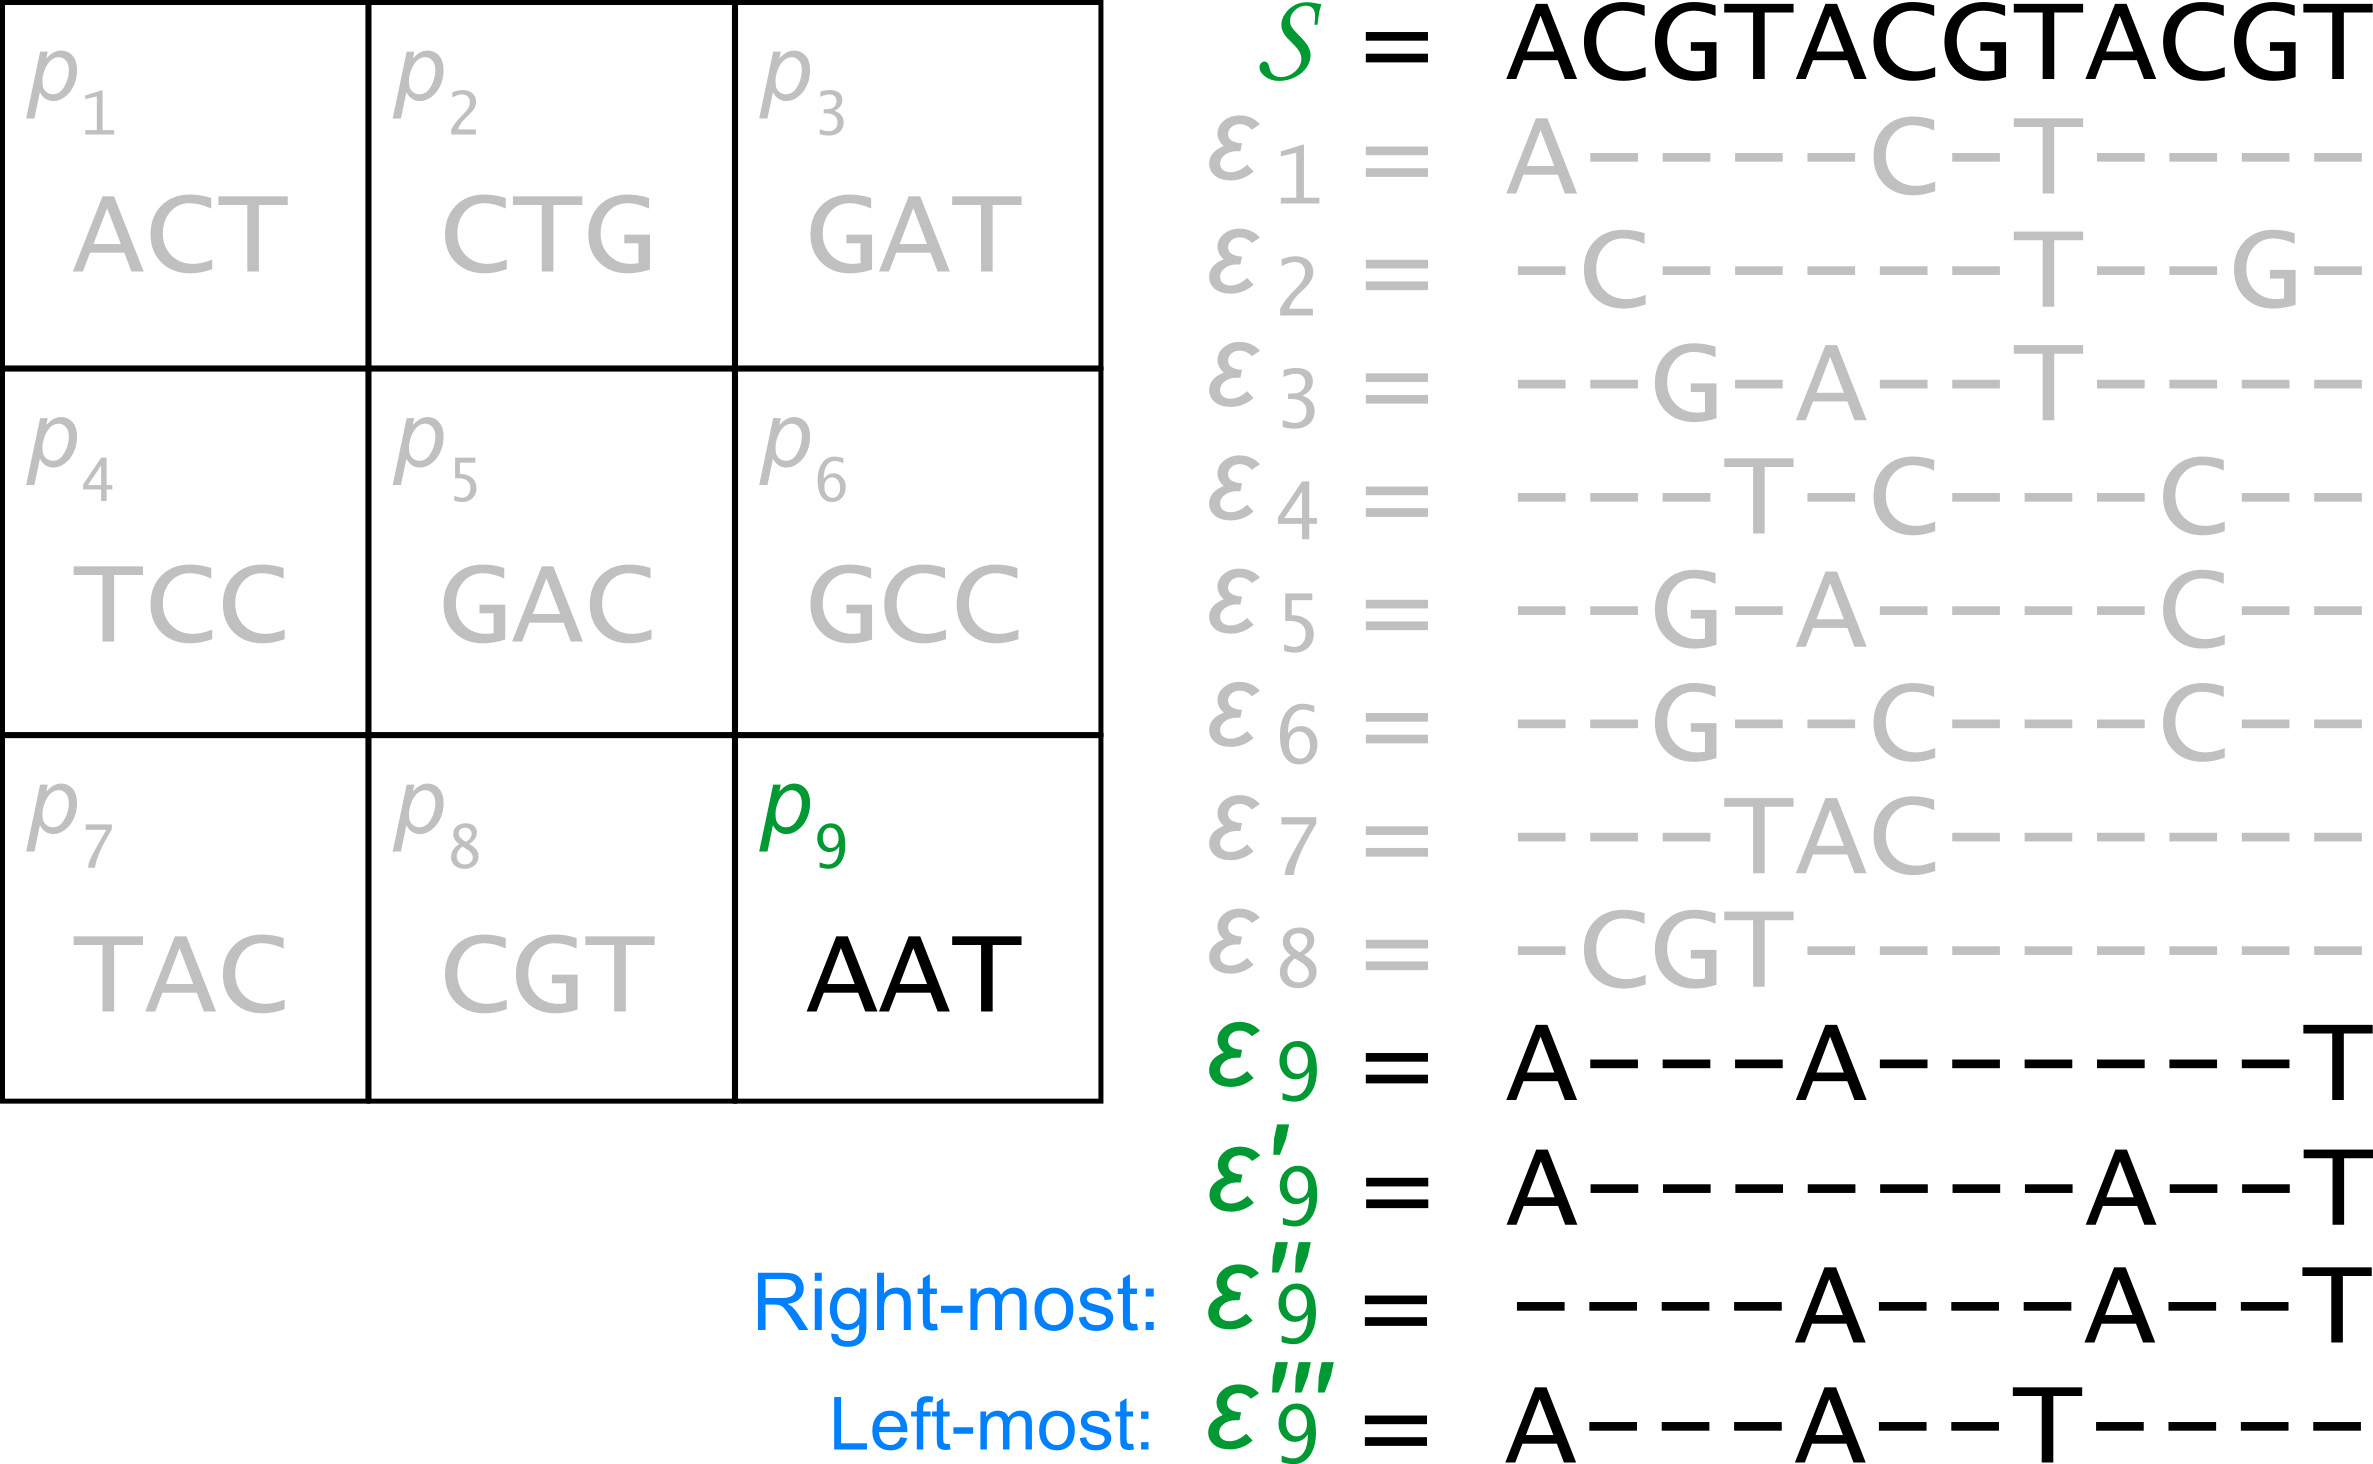
\includegraphics[width=\textwidth]{masks/alternatives.jpg}
  \end{overprint}

}

%%%%%%%%%%%%%%%%%%%%%%%%%%%%%%%%%%%%%%%%%%%%%%%%%%%%%%%%%%%%%%%%%%%%%%%%%%%%%%%%
\frame[label=problem]{\frametitle{Unintended Illumination Problem}

  \begin{columns}
  
    \begin{column}{0.45\textwidth}
      \centerline{
        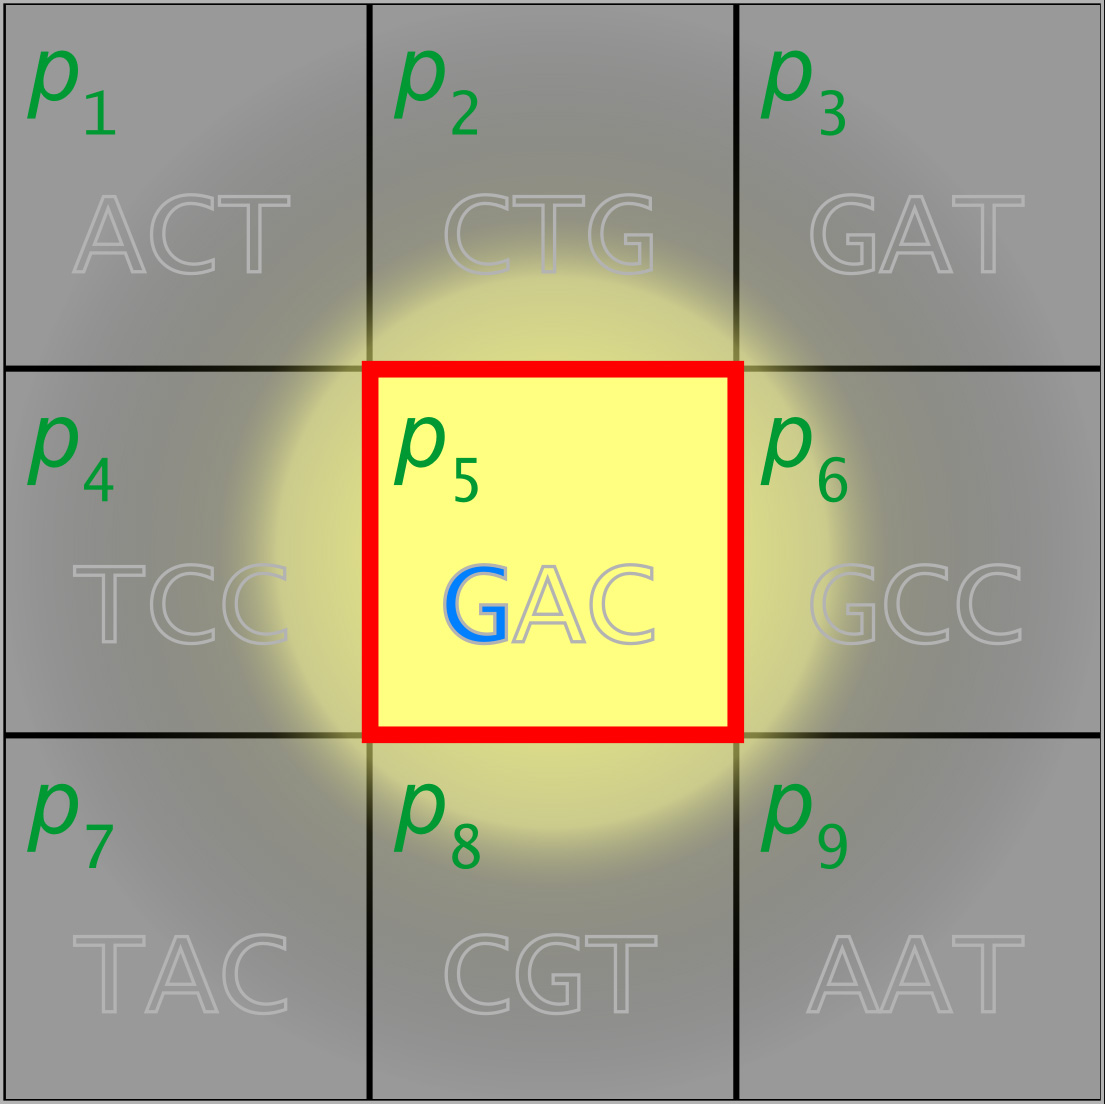
\includegraphics[width=\textwidth]{pics/straylight.jpg}
      }
    \end{column}
    
    \begin{column}{0.55\textwidth}
      \begin{itemize}
        \item \alert{Untargeted spots} can be accidentally activated
        \begin{itemize}
          \item Diffraction of light
          \item Internal reflection
        \end{itemize}
        \item Production of defective probes
        \item More likely near the \alert{borders} between masked and unmasked
              spots: \alert{border conflict}
      \end{itemize}
    \end{column}
    
  \end{columns}
  
  \begin{block}{Border Length Minimization Problem (Hannenhalli et al., 2002)}
    Find arrangement of the probes and embeddings with minimum number of border
    conflicts over all masks
  \end{block}

}

%% *****************************************************************************
\section[Conflict Index]{Conflict Index Model}
\subsection{Dummy}
%% *****************************************************************************

%%%%%%%%%%%%%%%%%%%%%%%%%%%%%%%%%%%%%%%%%%%%%%%%%%%%%%%%%%%%%%%%%%%%%%%%%%%%%%%%
\frame{\frametitle{Motivation}

  \begin{columns}  
  
    \begin{column}{0.55\textwidth}
      \begin{itemize}
        \item Border Length measures the quality of a particular mask
        \begin{itemize}
          \item We are more interested in a \alert{per-probe measure}
        \end{itemize}
        \item Practical considerations:
        \begin{itemize}
          \item[a)] Stray light might damage probes as far as \alert{three cells
                    away} from the targeted spot
          \item[b)] Imperfections \alert{in the middle} of a probe are more
                    harmful than in its extremities
        \end{itemize}
      \end{itemize}
    \end{column}
      
    \begin{column}{0.45\textwidth}
      \centerline{
        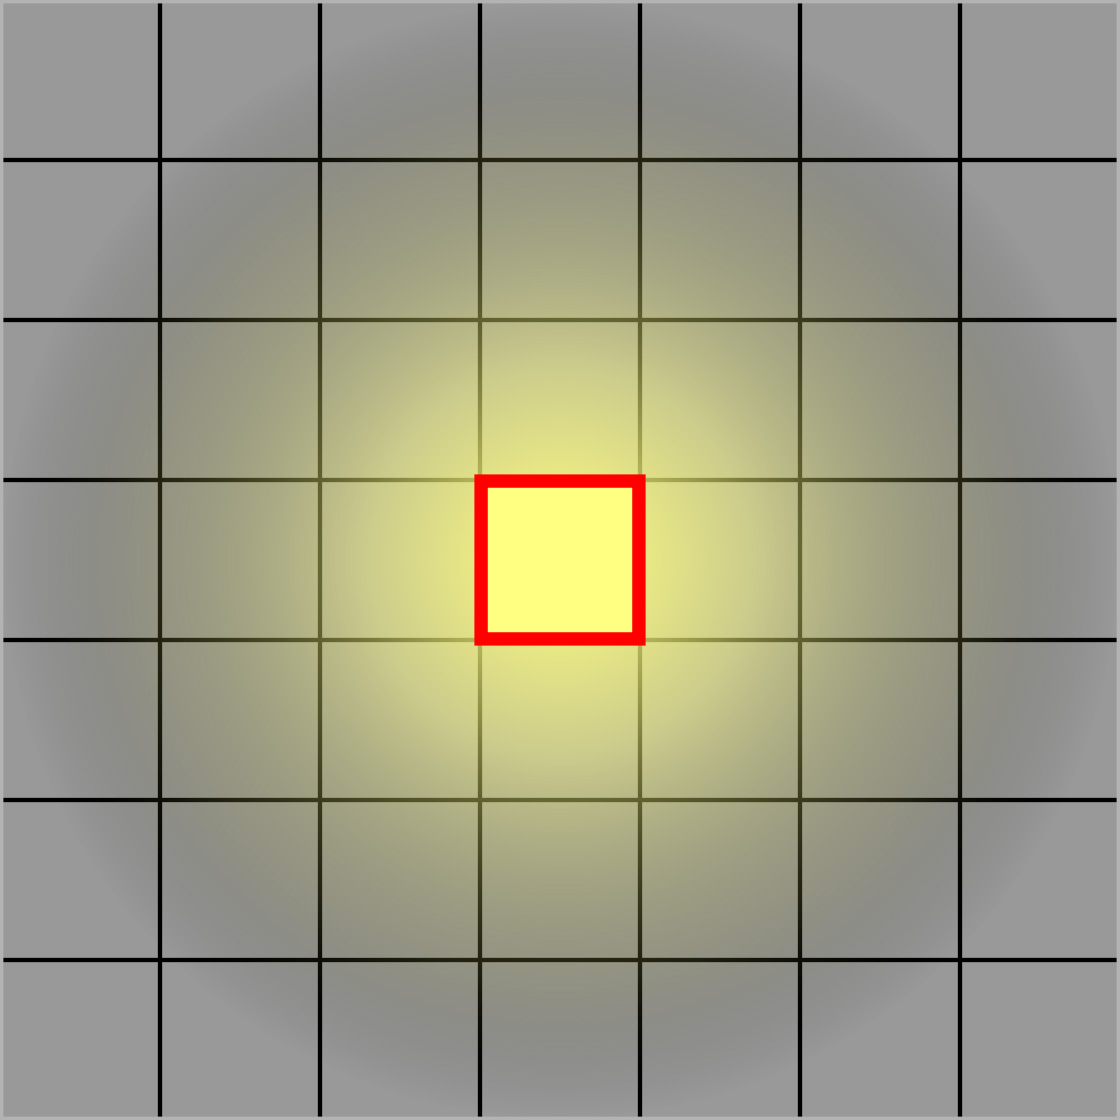
\includegraphics[width=\textwidth]{pics/distance.jpg}
      }
    \end{column}
  
  \end{columns}
  
  \vspace*{0.35cm}
  
\includegraphics[width=\textwidth]{pics/position.jpg}
}

%%%%%%%%%%%%%%%%%%%%%%%%%%%%%%%%%%%%%%%%%%%%%%%%%%%%%%%%%%%%%%%%%%%%%%%%%%%%%%%%
\frame{\frametitle{Definition}

  \begin{block}{Conflict Index of a probe $p$}
    \footnotesize{
    \[
    \mathcal{C}(p) := \sum_{t=1}^{T} \Bigl( \omega(p,t) \sum_{nbs. p'} \delta(p,p',t) \Bigr)
    \]
    }
  \end{block}
    
  \begin{block}{Distance-dependent weights}
    \footnotesize{
    \[
    \delta(p,p',t) :=
    \left\{
    \begin{array}{ll}
    (d(p,p'))^{-2} & \mbox{if $p'$ is unmasked at step $t$}, \\
                 0 & \mbox{otherwise}, \\
    \end{array}
    \right.
    \]
    %%
    where $d(p,p')$ is the \alert{Euclidean distance} between the spots of~$p$
    and~$p'$.
    }
  \end{block}

  \vspace*{0.2cm}

  \centerline{
  \scriptsize{
  \begin{tabular}{|c|c|c|c|c|c|c|c|} \hline
  0.06 & 0.08 & 0.10 & 0.11 & 0.10 & 0.08 & 0.06 \\ \hline
  0.08 & 0.13 & 0.20 & 0.25 & 0.20 & 0.13 & 0.08 \\ \hline
  0.10 & 0.20 & 0.50 & 1.00 & 0.50 & 0.20 & 0.10 \\ \hline
  0.11 & 0.25 & 1.00 & \alert{$p$} & 1.00 & 0.25 & 0.11 \\ \hline
  0.10 & 0.20 & 0.50 & 1.00 & 0.50 & 0.20 & 0.10 \\ \hline
  0.08 & 0.13 & 0.20 & 0.25 & 0.20 & 0.13 & 0.08 \\ \hline
  0.06 & 0.08 & 0.10 & 0.11 & 0.10 & 0.08 & 0.06 \\ \hline
  \end{tabular}}}
  
}

%%%%%%%%%%%%%%%%%%%%%%%%%%%%%%%%%%%%%%%%%%%%%%%%%%%%%%%%%%%%%%%%%%%%%%%%%%%%%%%%
\frame{\frametitle{Definition}

  \begin{columns}
  
    \begin{column}{0.45\textwidth}
      \begin{block}{Conflict Index of a probe $p$}
        \footnotesize{
        \[
        \mathcal{C}(p) := \sum_{t=1}^{T} \Bigl( \omega(p,t) \sum_{p'} \delta(p,p',t) \Bigr)
        \]
        }
      \end{block}
    \end{column}
    
    \begin{column}{0.45\textwidth}
      \centerline{
        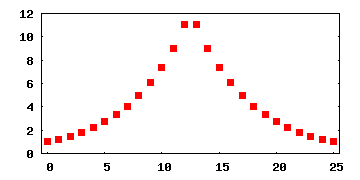
\includegraphics[width=1.25\textwidth]{pics/position_weights.png}
      }
    \end{column}
    
  \end{columns}

  \begin{block}{Position-dependent weights}
    \footnotesize{
    \[
    \omega(p,t) :=
    \left\{
    \begin{array}{ll}
    c \cdot \exp{\left(\theta \cdot \lambda(p,t)\right)} & \mbox{if $p$ is masked at step $t$}, \\
    0 & \mbox{otherwise}, \\
    \end{array}
    \right.
    \]
    %%
    where
    %%
    \[
    \lambda(p,t) := 1 + \min(b_{p,t},\ell_{p} - b_{p,t}),
    \]
    %%
    $b_{p,t}$ denotes the number of nucleotides synthesized up to and including
    step~$t$, $\ell_{p}$ is the length of probe~$p$, $c>0$ and $\theta>0$ are
    constants.
    }
  \end{block}

}

%%%%%%%%%%%%%%%%%%%%%%%%%%%%%%%%%%%%%%%%%%%%%%%%%%%%%%%%%%%%%%%%%%%%%%%%%%%%%%%%
\frame{\frametitle{Border Length and Conflict Index}

  \begin{block}{Redefine $\delta$ and $\omega$ as}
    \footnotesize{
    \[
    \delta(p,p',t) :=
    \left\{
    \begin{array}{ll}
    1 & \mbox{if $p'$ is a direct neighbor of $p$}\\
      & \mbox{and is unmasked at step $t$}, \\
    0 & \mbox{otherwise} \\
    \end{array}
    \right.
    \]
    %%
    \[
    \omega(p,t) :=
    \left\{
    \begin{array}{ll}
    1/2 & \mbox{if $p$ is masked at step $t$}, \\
    0   & \mbox{otherwise} \\
    \end{array}
    \right.
    \]
    }
  \end{block}
  
  \begin{itemize}
    \item Then $\sum_p\,\mathcal{C}(p) = \sum_{t=1}^T\, \mathcal{B}_t$
    \item Total border length can be modeled as total conflict index for a
          particular choice of $\delta$ and $\omega$
    \item For our choices, they are not equivalent but still \alert{correlated}
    \begin{itemize}
      \item A good layout has low border lengths and conflict indices
    \end{itemize}
  \end{itemize}

}

%%%%%%%%%%%%%%%%%%%%%%%%%%%%%%%%%%%%%%%%%%%%%%%%%%%%%%%%%%%%%%%%%%%%%%%%%%%%%%%%
\frame{\frametitle{New Problem}

  \begin{block}{Conflict Index Minimization Problem}
    Find placement of the probes and embeddings such that
    \footnotesize{
    \[
    \sum_{p} \mathcal{C}(p) \to \min
    \]
    }
  \end{block}

}


%% *****************************************************************************
\section[QAP Formulation]{New Approach: Quadratic Assignment Problem (QAP)}
\subsection{Dummy}
%% *****************************************************************************

%%%%%%%%%%%%%%%%%%%%%%%%%%%%%%%%%%%%%%%%%%%%%%%%%%%%%%%%%%%%%%%%%%%%%%%%%%%%%%%%
\frame{\frametitle{Previous Work: Place and Re-embed}

  The problem has been traditionally approached in two phases:
  \begin{itemize}
    \item[1)] \alert{Placement} of probes given a fixed embedding
    \item[2)] \alert{Re-embedding} of probes once a placement is fixed
  \end{itemize}
  
  \begin{block}{Placement: Row-epitaxial (Kahng {\it et~al}., 2003)}
    \begin{itemize}
      \item Spots are filled in a pre-defined order
      \begin{itemize}
        \item Select probe from a list $Q$ such that conflicts with filled spots
              are minimized
      \end{itemize}
      \item Restrict the maximum size of $Q$ (e.g. $Q = 20\,000$)
    \end{itemize}
  \end{block}

  \begin{block}{Re-embedding: several algorithms (Kahng {\it et~al}., 2002, 2003)}
    \begin{itemize}
      \item Based on the Optimum Single Probe Embedding (OSPE)
      \begin{itemize}
        \item Re-embed a probe \alert{optimally} in regards to its neighbors
        \item Dynamic programming, like a sequence alignment
      \end{itemize}
    \end{itemize}
  \end{block}
  
}

%%%%%%%%%%%%%%%%%%%%%%%%%%%%%%%%%%%%%%%%%%%%%%%%%%%%%%%%%%%%%%%%%%%%%%%%%%%%%%%%
\frame{\frametitle{Previous Work: Partitioning}

  \begin{itemize}
    \item The placement problem can be \alert{partitioned}
    \begin{itemize}
      \item Divide the chip into sub-regions; assign sub-sets of probes to each
            sub-region
      \item Sub-regions are processed independently, and can be
            \alert{recursively partitioned}
      \item A placement algorithm is called on each final sub-region
    \end{itemize}
  \end{itemize}

  \begin{block}{Pivot Partitioning (Carvalho \& Rahmann, 2006)}
    \begin{itemize}
      \item Alternate \alert{horizontal} and \alert{vertical} partitions
      \item Allow sub-regions to have different sizes
    \end{itemize}
  \end{block}

  \vspace*{0.25cm}
  
  \centerline{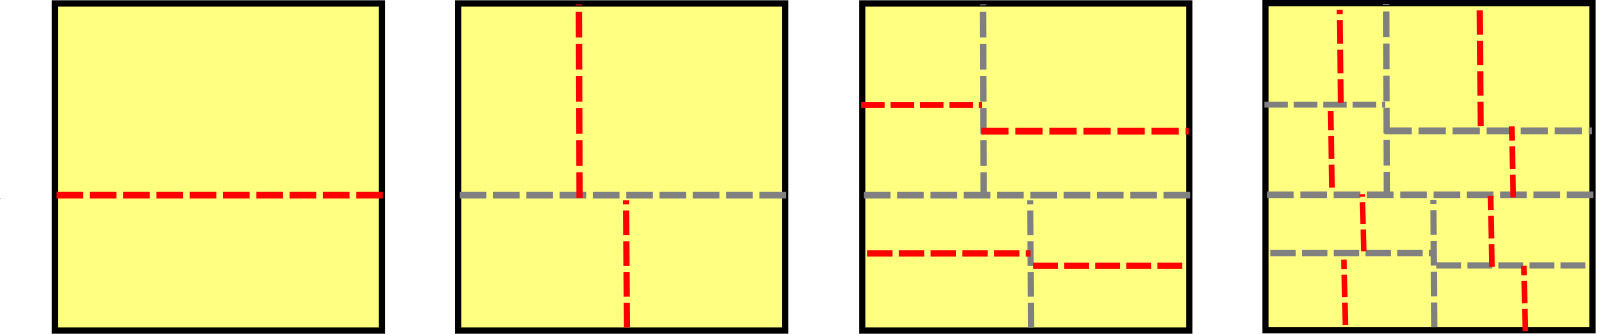
\includegraphics[width=0.8\textwidth]{pics/pivotpart.jpg}}
  
  %% \item Partitioning is a compromise but can reduce run-time and help the
  %% placement algorithm

}

%%%%%%%%%%%%%%%%%%%%%%%%%%%%%%%%%%%%%%%%%%%%%%%%%%%%%%%%%%%%%%%%%%%%%%%%%%%%%%%%
\frame{\frametitle{Quadratic Assignment Problem (QAP)}

  \begin{block}{Definition}
    \begin{itemize}
      \item Given $n \times n$ real-valued matrices $F = (f_{ij})\geq 0$ and
            $D = (d_{kl})\geq 0$
      \item Find a permutation $\pi$ of $\{1, 2, \ldots n\}$ such that
    \end{itemize}
    \footnotesize{
    \[
      \sum_{i=1}^{n} \sum_{j=1}^{n}\,  f_{ij} \cdot d_{\pi(i)\pi(j)} \to \min
    \]
    }
  \end{block}

  \begin{block}{Example: Facility Location Problem }
    \begin{itemize}
      \item Assign $n$ \alert{facilities} to $n$ \alert{locations}
      \item $f_{ij}$: \alert{flow} of materials from facility $i$ to $j$
      \item $d_{kl}$: \alert{distance} between locations $k$ and $l$
      \item $\pi$: one-to-one assignment with minimum cost
    \end{itemize}
  \end{block}

}


%%%%%%%%%%%%%%%%%%%%%%%%%%%%%%%%%%%%%%%%%%%%%%%%%%%%%%%%%%%%%%%%%%%%%%%%%%%%%%%%
\frame{\frametitle{QAP Formulation of Placement Problem}

  \begin{block}{QAP}
    \begin{itemize}
      \item Given $n \times n$ real-valued matrices $F$ and $D$
      \item Find a permutation $\pi$ of $\{1, 2, \ldots n\}$ such that
    \end{itemize}
    \footnotesize{
    \[
      \sum_{i=1}^{n} \sum_{j=1}^{n}\,  f_{ij} \cdot d_{\pi(i)\pi(j)} \to \min
    \]
    }
  \end{block}

  \begin{block}{Placement as a QAP}
    \begin{itemize}
      \item Given a set of probes with \alert{fixed} embeddings
      \item Find \alert{placement} on the chip such that
    \end{itemize}
    \footnotesize{
    \[
      \sum_{k} \mathcal{C}(k) \to \min
    \]
    }
  \end{block}

}

%%%%%%%%%%%%%%%%%%%%%%%%%%%%%%%%%%%%%%%%%%%%%%%%%%%%%%%%%%%%%%%%%%%%%%%%%%%%%%%%
\frame{\frametitle{QAP Formulation of Placement Problem}

  \begin{block}{Goal: find a placement with}
    \footnotesize{
    \[
      \sum_{k} \mathcal{C}(k) \to \min
    \]
    }
  \end{block}

  \begin{block}{``Flow'' $f_{ij}$: distance between spots $i$ and $j$}
    \footnotesize{
    \[
    f_{ij} :=
    \left\{
    \begin{array}{ll}
    (d(i,j))^{-2} & \mbox{if spot $j$ is ``near'' spot $i$,} \\
                0 & \mbox{otherwise} \\
    \end{array}
    \right.
    \]
    }
  \end{block}

  \begin{block}{``Distance'' $d_{kl}$: conflicts between probes $k$ and $l$}
    \footnotesize{
    \[
      d_{kl} := \sum_{t=1}^T\, d_{klt},
    \]
    }
    %%
    \footnotesize{
    \[
      d_{klt} := \left\{ \begin{array}{ll}
      c \cdot \exp(\theta \cdot \lambda(k,t)) 
        & \mbox{if $k$ is masked and $l$ unmasked in step $t$,}\\
      0 & \mbox{otherwise}
      \end{array} \right.
    \]
    }
  \end{block}

}

%%%%%%%%%%%%%%%%%%%%%%%%%%%%%%%%%%%%%%%%%%%%%%%%%%%%%%%%%%%%%%%%%%%%%%%%%%%%%%%%
\frame{\frametitle{QAP Heuristics}

  \begin{itemize}
    \item The placement problem can be modeled as a QAP
    \item But QAP is known to be NP-hard
    \begin{itemize}
      \item Generally impossible to solve (to optimality) for $n \geq 20$
    \end{itemize}
    \item Several \alert{heuristics} exist
  \end{itemize}

  \begin{block}{GRASP (Li, Pardalos and Resende, 1994)}
    \begin{itemize}
      \item Greedy Randomized Adaptive Search Procedure
      \item Comprised of two phases
      \begin{itemize}
        \item[1)] Construction: builds a random feasible solution
        \item[2)] Local search: search a local optimum in the neighborhood
      \end{itemize}
      \item GRASP with Path-Relinking (Oliveira {\it et~al}., 2004)
    \end{itemize}
  \end{block}

}

%%%%%%%%%%%%%%%%%%%%%%%%%%%%%%%%%%%%%%%%%%%%%%%%%%%%%%%%%%%%%%%%%%%%%%%%%%%%%%%%
\frame{\frametitle{Results on Small Artificial Chips}

  \begin{block}{Border Length minimization}
    \scriptsize{
    \centerline{
    \begin{tabular}{c|r|rrr|rrr}
    & Random & \multicolumn{3}{|c}{Row-epitaxial} & \multicolumn{3}{|c}{GRASP with Path-Relinking}  \\ \noalign{\smallskip} \cline{2-8} \noalign{\smallskip}
Dim & Cost   & Cost & Red. & Time & Cost & Red. & Time \\ \noalign{\smallskip} \hline \noalign{\smallskip}
6$\times$6   & 1\,989.20 & 1\,714.60 & 13.80 & 0.01 & \color{green!85!black} 1\,672.20 & \color{green!85!black} 15.94 & \color{red}    2.73 \\
7$\times$7   & 2\,783.20 & 2\,354.60 & 15.40 & 0.02 & \color{green!85!black} 2\,332.60 & \color{green!85!black} 16.19 & \color{red}    6.43 \\
8$\times$8   & 3\,721.20 & 3\,123.80 & 16.05 & 0.03 & \color{green!85!black} 3\,099.13 & \color{green!85!black} 16.72 & \color{red}  12.49 \\
9$\times$9   & 4\,762.00 & 3\,974.80 & 16.53 & 0.05 & \color{green!85!black} 3\,967.20 & \color{green!85!black} 16.69 & \color{red}  25.96 \\
10$\times$10 & 5\,985.20 & 4\,895.60 & 18.20 & 0.06 & \color{red}            4\,911.40 & \color{red}            17.94 & \color{red}  47.57 \\
11$\times$11 & 7\,288.40 & 5\,954.40 & 18.30 & 0.10 & \color{red}            5\,990.73 & \color{red}            17.80 & \color{red}  87.48 \\
12$\times$12 & 8\,714.00 & 7\,086.20 & 18.68 & 0.11 & \color{red}            7\,159.80 & \color{red}            17.84 & \color{red} 152.42 \\
    \end{tabular}}
    }
  \end{block}
  
  \scriptsize{
    Dim: chip dimension \\
    Cost: \alert{total border length} \\
    Red.: reduction in \% \\
    Time: running time in seconds
  }
  
}

%%%%%%%%%%%%%%%%%%%%%%%%%%%%%%%%%%%%%%%%%%%%%%%%%%%%%%%%%%%%%%%%%%%%%%%%%%%%%%%%
\frame{\frametitle{Results on Small Artificial Chips}

  \begin{block}{Conflict Index minimization}
    \scriptsize{
    \centerline{
    \begin{tabular}{c|r|rrr|rrr}
    & Random & \multicolumn{3}{|c}{Row-epitaxial} & \multicolumn{3}{|c}{GRASP with Path-Relinking}  \\ \noalign{\smallskip} \cline{2-8} \noalign{\smallskip}
Dim & Cost   & Cost & Red. & Time & Cost & Red. & Time \\ \noalign{\smallskip} \hline \noalign{\smallskip}
6$\times$6   & 524.28 & 495.15 & 5.56 & 0.05 & \color{green!85!black} 467.08 & \color{green!85!black} 10.91 & \color{red}   3.68 \\
7$\times$7   & 558.25 & 521.90 & 6.51 & 0.07 & \color{green!85!black} 489.32 & \color{green!85!black} 12.35 & \color{red}   8.84 \\
8$\times$8   & 590.51 & 551.84 & 6.55 & 0.09 & \color{green!85!black} 515.69 & \color{green!85!black} 12.67 & \color{red}  19.48 \\
9$\times$9   & 613.25 & 568.62 & 7.28 & 0.11 & \color{green!85!black} 533.79 & \color{green!85!black} 12.96 & \color{red}  38.83 \\
10$\times$10 & 628.50 & 576.49 & 8.28 & 0.11 & \color{green!85!black} 539.69 & \color{green!85!black} 14.13 & \color{red}  73.09 \\
11$\times$11 & 642.72 & 588.91 & 8.37 & 0.12 & \color{green!85!black} 551.41 & \color{green!85!black} 14.21 & \color{red} 145.67 \\
12$\times$12 & 656.86 & 598.21 & 8.93 & 0.12 & \color{green!85!black} 561.21 & \color{green!85!black} 14.56 & \color{red} 249.19 \\
    \end{tabular}}
    }
  \end{block}

  \scriptsize{
    Dim: chip dimension \\
    Cost: \alert{average conflict index} \\
    Red.: reduction in \% \\
    Time: running time in seconds
  }

}

%%%%%%%%%%%%%%%%%%%%%%%%%%%%%%%%%%%%%%%%%%%%%%%%%%%%%%%%%%%%%%%%%%%%%%%%%%%%%%%%
\frame{\frametitle{Applications}

  \begin{columns}
  
    \begin{column}{0.60\textwidth}
      \begin{itemize}
        \item QAP is good for small regions...
        \begin{itemize}
          \item But not feasible for an entire microarray chip
        \end{itemize}
        \onslide+<2->
        \item Two applications:
          \begin{itemize}
            \item[1)] Combine it with a \alert{partitioning algorithm}
            \onslide+<3->
            \item[2)] Use it as a \alert{post-placement} optimization inside a
                      sliding-window
          \end{itemize}
      \end{itemize}
    \end{column}

    \begin{column}{0.40\textwidth}
      \begin{overprint}
        \onslide+<3>\centerline{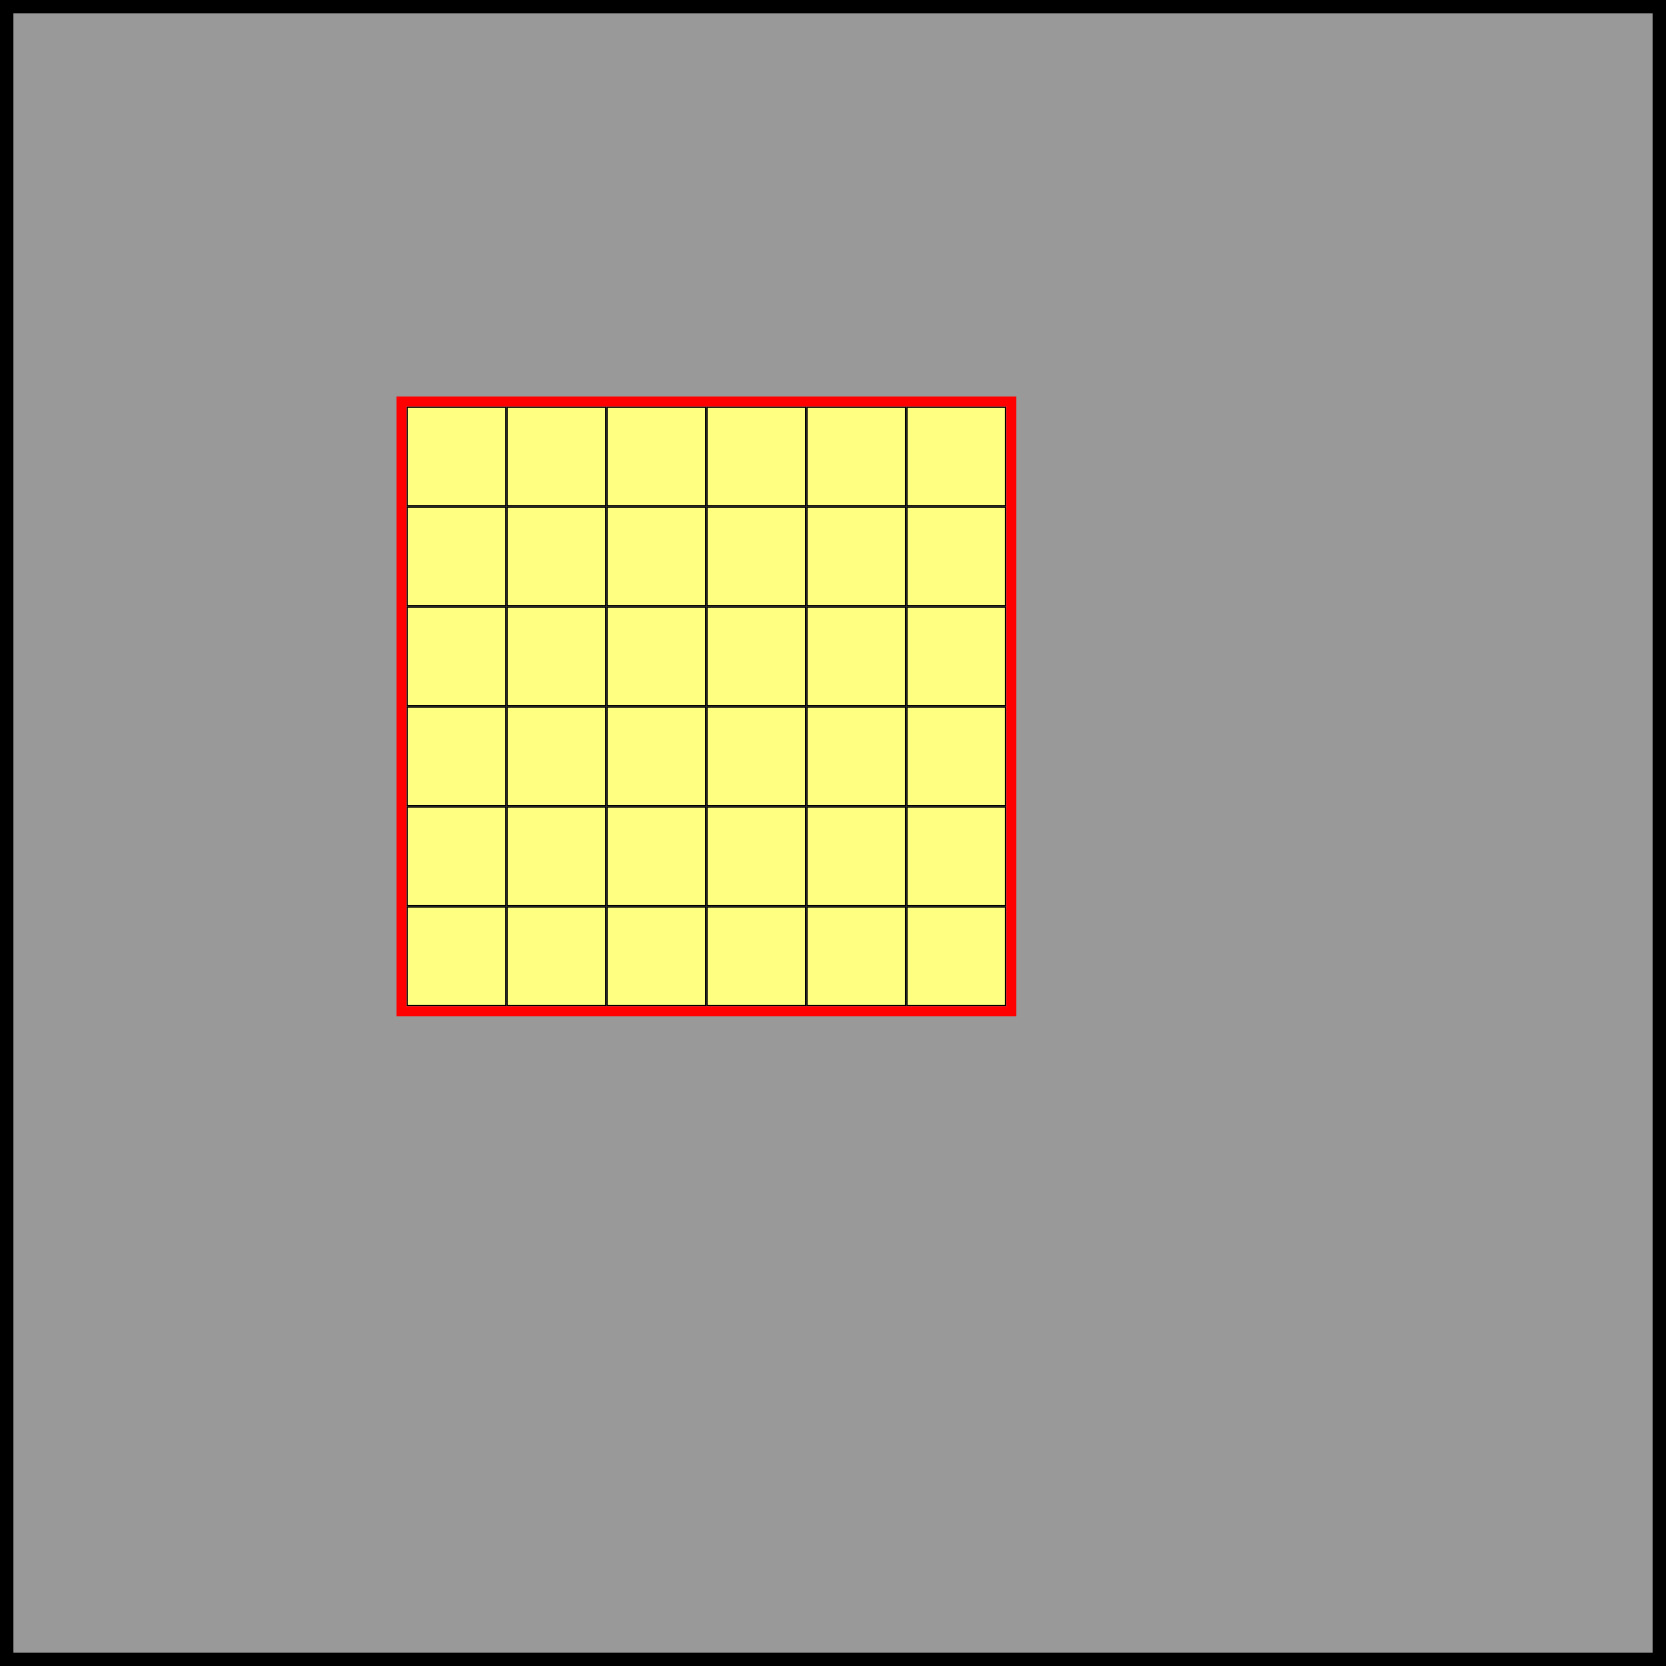
\includegraphics[width=\textwidth]{pics/optimization1.jpg}}
        \onslide+<4->\centerline{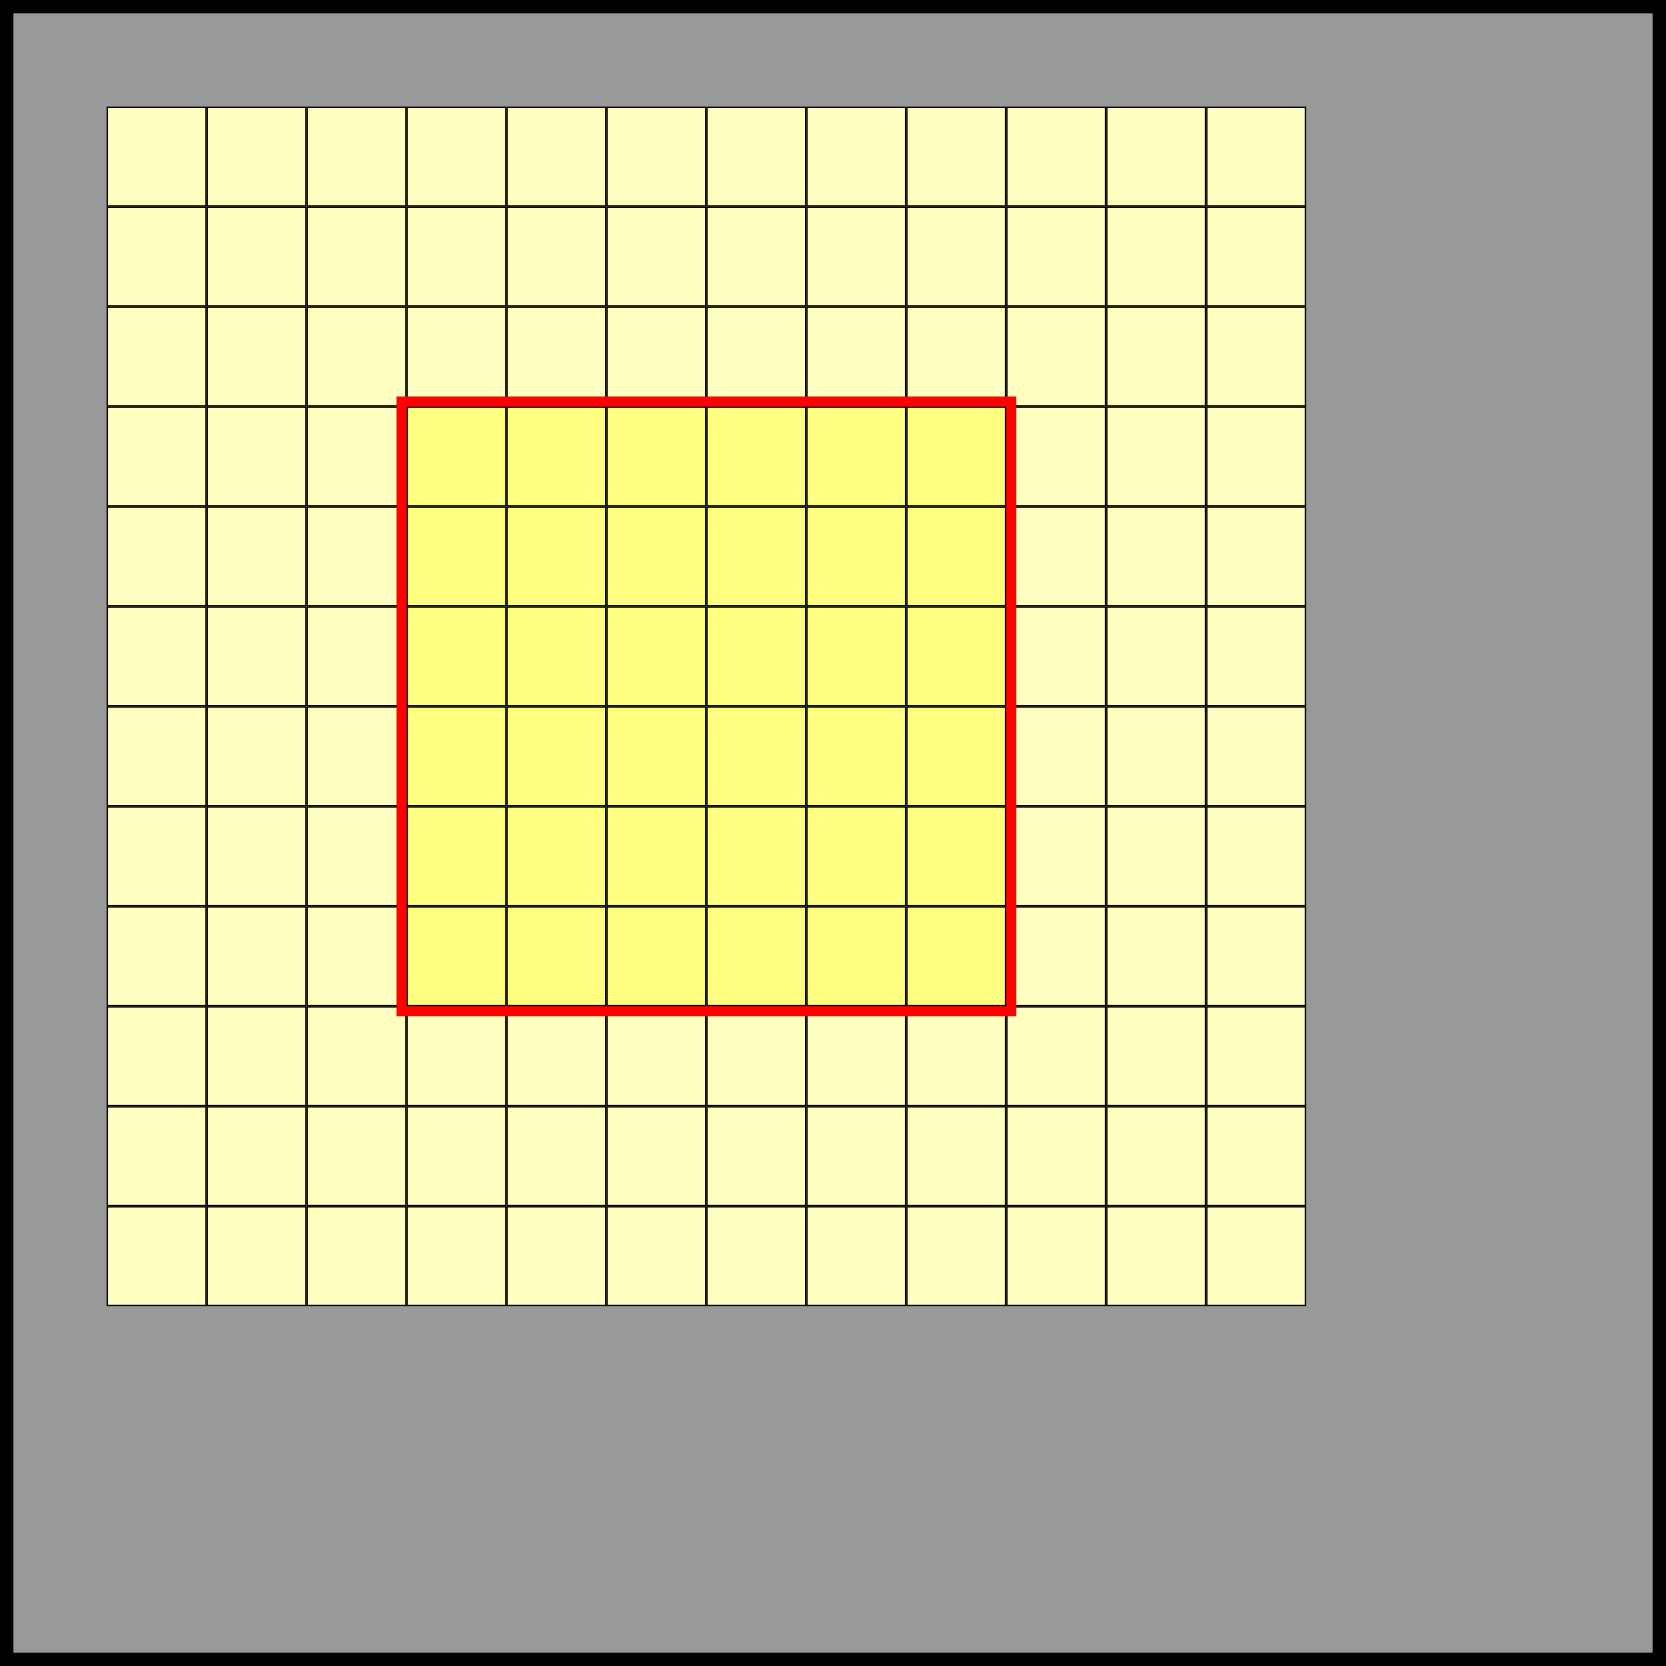
\includegraphics[width=\textwidth]{pics/optimization2.jpg}}
      \end{overprint}
    \end{column}
    
  \end{columns}
  
  \vspace*{0.3cm}
  
  \onslide+<2->\centerline{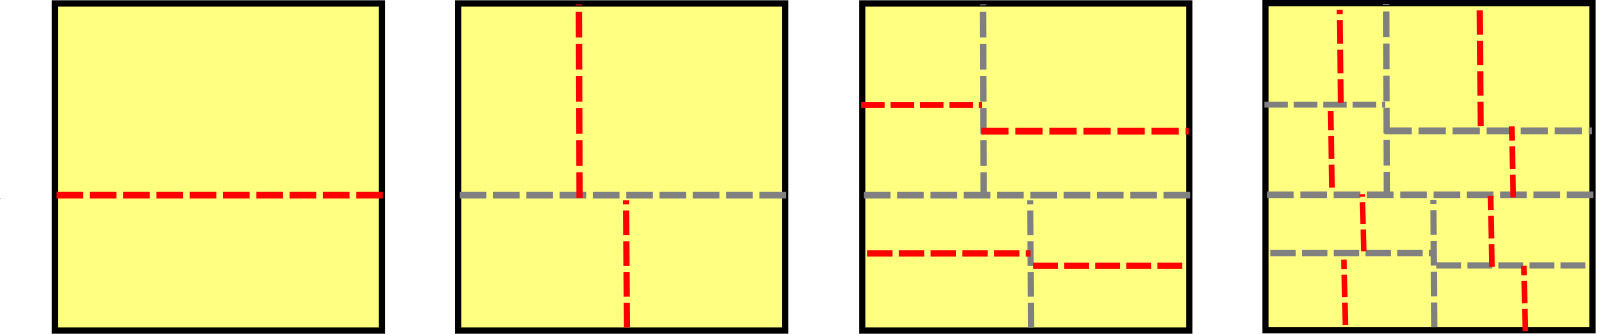
\includegraphics[width=0.8\textwidth]{pics/pivotpart.jpg}}

}

%% *****************************************************************************
\section*{Summary}
\subsection*{Dummy}
%% *****************************************************************************

%%%%%%%%%%%%%%%%%%%%%%%%%%%%%%%%%%%%%%%%%%%%%%%%%%%%%%%%%%%%%%%%%%%%%%%%%%%%%%%%
\frame{\frametitle{Summary}

  \begin{itemize}
    \item \alert{Conflict Index}
    \begin{itemize}
      \item New model for evaluating microarray layouts
    \end{itemize}
    \item \alert{New approach to placement}
    \begin{itemize}
      \item Based on the Quadratic Assignment Problem
    \end{itemize}
  \end{itemize}
  
  \vspace*{0.3cm}
  \begin{itemize}
    \item Challenges
    \begin{itemize}
      \item Faster or better QAP heuristics?
      \item Adapt QAP for post-placement optimization
      \item Formulation considering all embeddings
    \end{itemize}
  \end{itemize}

}

%%%%%%%%%%%%%%%%%%%%%%%%%%%%%%%%%%%%%%%%%%%%%%%%%%%%%%%%%%%%%%%%%%%%%%%%%%%%%%%%
\frame{\frametitle{Auf Wiedersehen!}

  \begin{block}{More info on}
    \centerline{\tt\alert{
      http://gi.cebitec.uni-bielefeld.de/assb/chiplayout
    }}
  \end{block}

  \begin{block}{QAPLIB}
    \centerline{\tt\alert{
      http://www.seas.upenn.edu/qaplib
    }}
  \end{block}

  \begin{itemize}
    \item Thanks to Peter Hahn (University of Pennsylvania, USA)
    \item And \alert{thank you} for your attention!
  \end{itemize}
  
}

\end{document}
